\chapter{Figures with matlab2tikz}

\lipsum[1-3]
\pagebreak
\lstinputlisting[caption={A simple example of 2 similar figures and exporting them with matlab2tikz. For each figure there will be a tex file with a standalone version that can be quickly be translated to pdf and from there to svg (a foss vector image format) and emf (vector image format for Windows). There is a small bash script for that job available \texttt{convert\_pdf2svg2emf.sh}}, label=Beispiel0]{Beispiel0.m}


\begin{figure}[H]
	\centering
	% This file was created by matlab2tikz.%
%
\definecolor{mycolor1}{rgb}{0.00000,0.44706,0.69804}%
\definecolor{mycolor2}{rgb}{0.90196,0.62353,0.00000}%
%
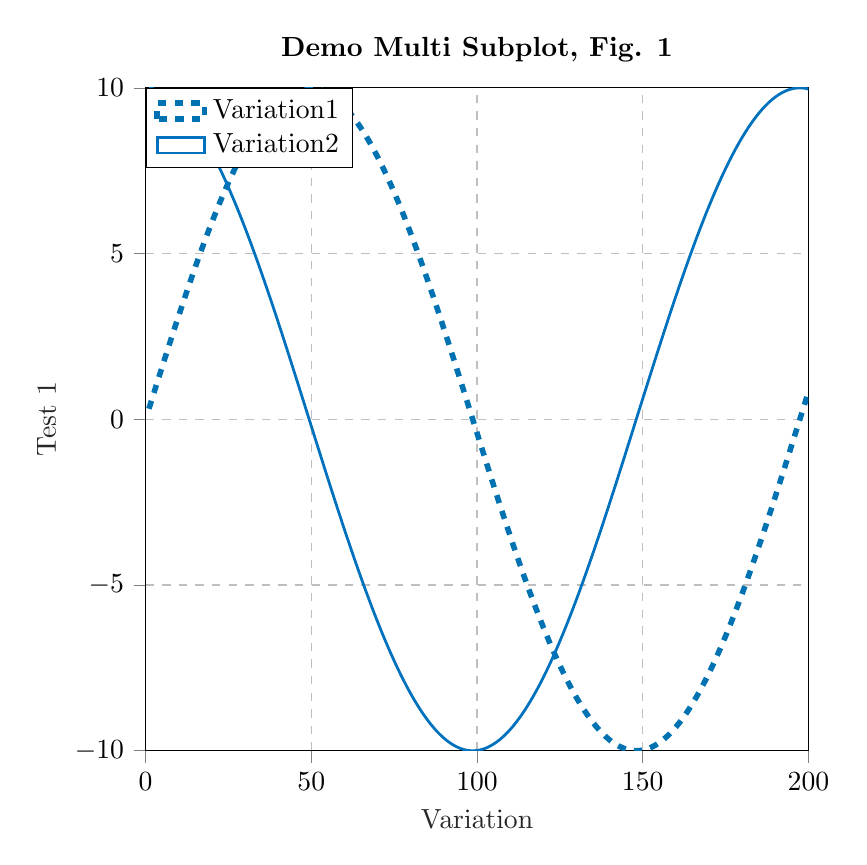
\begin{tikzpicture}

\begin{axis}[%
xmin=0,
xmax=200,
tick align=outside,
xlabel style={font=\color{white!15!black}},
xlabel={Variation},
ymin=-10,
ymax=10,
ylabel style={font=\color{white!15!black}},
ylabel={Test 1},
axis background/.style={fill=white},
title style={font=\bfseries},
title={Demo Multi Subplot, Fig. 1},
xmajorgrids,
xminorgrids,
ymajorgrids,
yminorgrids,
grid style={dashed},
x tick label style={/pgf/number format/.cd, fixed, fixed zerofill, precision=0, /tikz/.cd},
y tick label style={/pgf/number format/.cd, fixed, fixed zerofill, precision=0, /tikz/.cd},
xtick={0,50,100,150,200},
ytick={-10,-5,0,5,10},
ytick pos=left,
xtick pos=bottom,
/pgf/number format/.cd, set decimal separator={.},
/pgf/number format/.cd, 1000 sep={},
legend style={at={(0,1)}, anchor=north west},
legend cell align={left},
at={(0cm,0cm)},
height=10cm,
width=10cm
]
\addplot [color=mycolor1, dashed, line width=2.0pt]
  table[row sep=crcr]{%
1	0.318256136349473\\
2	0.636189839040428\\
3	0.953479001080363\\
4	1.26980216847786\\
5	1.58483886591605\\
6	1.89826992143462\\
7	2.2097777897913\\
8	2.51904687417527\\
9	2.82576384594664\\
10	3.12961796207787\\
11	3.43030137997574\\
12	3.7275094693648\\
13	4.02094112091622\\
14	4.31029905130968\\
15	4.59529010441881\\
16	4.87562554831546\\
17	5.15102136779154\\
18	5.42119855210235\\
19	5.68588337763963\\
20	5.94480768524822\\
21	6.1977091519051\\
22	6.44433155648575\\
23	6.68442503934853\\
24	6.91774635547401\\
25	7.14405912090294\\
26	7.36313405222303\\
27	7.57474919886199\\
28	7.77869016795151\\
29	7.97475034153431\\
30	8.16273108589421\\
31	8.34244195279721\\
32	8.51370087243952\\
33	8.67633433790736\\
34	8.83017758096132\\
35	8.9750747389674\\
36	9.11087901280556\\
37	9.23745281559575\\
38	9.35466791209081\\
39	9.46240554859496\\
40	9.5605565732763\\
41	9.64902154675137\\
42	9.72771084282985\\
43	9.79654473931719\\
44	9.85545349878326\\
45	9.90437743921515\\
46	9.94326699448263\\
47	9.97208276455488\\
48	9.99079555541768\\
49	9.99938640865066\\
50	9.99784662063456\\
51	9.98617775136911\\
52	9.96439162289251\\
53	9.93251030730429\\
54	9.89056610440339\\
55	9.83860150896448\\
56	9.77666916768531\\
57	9.70483182584899\\
58	9.62316226375512\\
59	9.53174322298409\\
60	9.43066732256947\\
61	9.3200369651632\\
62	9.19996423328878\\
63	9.07057077578752\\
64	8.93198768457289\\
65	8.78435536181788\\
66	8.62782337770985\\
67	8.46255031891705\\
68	8.28870362792026\\
69	8.10645943337249\\
70	7.91600237165831\\
71	7.71752539983398\\
72	7.5112296001375\\
73	7.29732397626694\\
74	7.07602524163332\\
75	6.84755759980251\\
76	6.61215251734875\\
77	6.37004848934974\\
78	6.12149079776103\\
79	5.86673126291441\\
80	5.60602798839214\\
81	5.33964509953538\\
82	5.06785247585189\\
83	4.790925477594\\
84	4.50914466678392\\
85	4.22279552296894\\
86	3.93216815399462\\
87	3.63755700208891\\
88	3.33926054555497\\
89	3.03758099637498\\
90	2.73282399403119\\
91	2.42529829585458\\
92	2.11531546421465\\
93	1.80318955086743\\
94	1.48923677878134\\
95	1.17377522176344\\
96	0.857124482210443\\
97	0.539605367311188\\
98	0.221539564028375\\
99	-0.0967506868109106\\
100	-0.414942916985869\\
101	-0.732714757582999\\
102	-1.04974426559655\\
103	-1.36571025009741\\
104	-1.68029259764011\\
105	-1.99317259657816\\
106	-2.30403325995918\\
107	-2.61255964667274\\
108	-2.91843918052548\\
109	-3.22136196692024\\
110	-3.52102110681844\\
111	-3.81711300766757\\
112	-4.1093376909788\\
113	-4.39739909624303\\
114	-4.6810053808776\\
115	-4.9598692158997\\
116	-5.23370807702688\\
117	-5.50224453090987\\
118	-5.76520651620755\\
119	-6.02232761921949\\
120	-6.27334734379666\\
121	-6.51801137525691\\
122	-6.75607183803788\\
123	-6.98728754682626\\
124	-7.21142425090892\\
125	-7.42825487149853\\
126	-7.63755973179302\\
127	-7.8391267795359\\
128	-8.03275180185202\\
129	-8.21823863214097\\
130	-8.39539934881863\\
131	-8.5640544657055\\
132	-8.72403311386878\\
133	-8.87517321473428\\
134	-9.01732164429241\\
135	-9.15033438823219\\
136	-9.2740766878459\\
137	-9.38842317655668\\
138	-9.4932580069307\\
139	-9.58847496804528\\
140	-9.67397759309389\\
141	-9.74967925711929\\
142	-9.81550326477549\\
143	-9.87138292802986\\
144	-9.91726163372651\\
145	-9.95309290094258\\
146	-9.97884042807926\\
147	-9.99447812963992\\
148	-9.999990162658\\
149	-9.99537094274795\\
150	-9.98062514976289\\
151	-9.95576772305335\\
152	-9.92082384633183\\
153	-9.87582892215847\\
154	-9.82082853607387\\
155	-9.75587841041509\\
156	-9.68104434786193\\
157	-9.59640216477052\\
158	-9.50203761436175\\
159	-9.39804629984242\\
160	-9.28453357754716\\
161	-9.1616144501991\\
162	-9.02941345039764\\
163	-8.88806451445118\\
164	-8.73771084668271\\
165	-8.57850477434576\\
166	-8.41060759329765\\
167	-8.23418940458644\\
168	-8.04942894211705\\
169	-7.85651339157125\\
170	-7.65563820076495\\
171	-7.44700688163486\\
172	-7.23083080405519\\
173	-7.00732898169329\\
174	-6.77672785012114\\
175	-6.53926103740752\\
176	-6.29516912742324\\
177	-6.04469941609938\\
178	-5.78810566088518\\
179	-5.52564782365976\\
180	-5.2575918073579\\
181	-4.98420918657674\\
182	-4.7057769324365\\
183	-4.42257713197366\\
184	-4.13489670235125\\
185	-3.8430271001755\\
186	-3.54726402621343\\
187	-3.24790712581076\\
188	-2.94525968531321\\
189	-2.63962832479917\\
190	-2.33132268743488\\
191	-2.02065512576672\\
192	-1.70794038526872\\
193	-1.39349528546558\\
194	-1.07763839895449\\
195	-0.760689728650891\\
196	-0.442970383585066\\
197	-0.124802253578178\\
198	0.193492316872784\\
199	0.511590855170724\\
200	0.829171087323842\\
};
\addplot [color=mycolor2, line width=1.0pt]
  table[row sep=crcr]{%
1	9.9949343685527\\
2	9.97974260633518\\
3	9.95444010452114\\
4	9.91905249774034\\
5	9.87361563810755\\
6	9.81817555889976\\
7	9.75278842791871\\
8	9.67752049058579\\
9	9.59244800282706\\
10	9.49765715381639\\
11	9.3932439786549\\
12	9.27931426107532\\
13	9.15598342626967\\
14	9.02337642394901\\
15	8.88162760175355\\
16	8.73088056914156\\
17	8.57128805189482\\
18	8.40301173738817\\
19	8.22622211077973\\
20	8.04109828228792\\
21	7.84782780573018\\
22	7.6466064885073\\
23	7.43763819322575\\
24	7.22113463115915\\
25	6.99731514775799\\
26	6.766406500425\\
27	6.52864262878125\\
28	6.28426441765578\\
29	6.03351945303887\\
30	5.77666177124611\\
31	5.51395160154758\\
32	5.24565510252271\\
33	4.97204409240804\\
34	4.69339577371098\\
35	4.40999245236874\\
36	4.12212125173668\\
37	3.83007382169614\\
38	3.53414604317627\\
39	3.23463772838926\\
40	2.93185231708274\\
41	2.62609656911697\\
42	2.31768025367836\\
43	2.00691583544419\\
44	1.69411815801639\\
45	1.37960412494525\\
46	1.06369237866609\\
47	0.746702977674199\\
48	0.428957072265208\\
49	0.110776579169256\\
50	-0.20751614459131\\
51	-0.525598628290302\\
52	-0.84314861420127\\
53	-1.15984438408527\\
54	-1.47536508513206\\
55	-1.78939105502456\\
56	-2.10160414579709\\
57	-2.41168804615947\\
58	-2.71932860196031\\
59	-3.02421413446482\\
60	-3.32603575612475\\
61	-3.62448768352046\\
62	-3.91926754715817\\
63	-4.21007669780842\\
64	-4.49662050907548\\
65	-4.77860867589107\\
66	-5.05575550863007\\
67	-5.32778022255019\\
68	-5.59440722226238\\
69	-5.85536638094374\\
70	-6.11039331401015\\
71	-6.35922964697119\\
72	-6.60162327719617\\
73	-6.8373286293259\\
74	-7.06610690407158\\
75	-7.28772632014861\\
76	-7.50196234910031\\
77	-7.70859794277358\\
78	-7.90742375321615\\
79	-8.09823834477244\\
80	-8.28084839816332\\
81	-8.45506890634298\\
82	-8.62072336193442\\
83	-8.77764393605372\\
84	-8.92567164834188\\
85	-9.06465652803202\\
86	-9.19445776588867\\
87	-9.31494385686537\\
88	-9.42599273333583\\
89	-9.52749188876388\\
90	-9.61933849168681\\
91	-9.70143948989658\\
92	-9.77371170471354\\
93	-9.83608191525683\\
94	-9.8884869326265\\
95	-9.93087366392173\\
96	-9.96319916603073\\
97	-9.9854306891375\\
98	-9.99754570990151\\
99	-9.99953195427674\\
100	-9.99138740994679\\
101	-9.97312032836364\\
102	-9.94474921638787\\
103	-9.90630281753889\\
104	-9.8578200828741\\
105	-9.79935013152657\\
106	-9.73095220094118\\
107	-9.65269558685952\\
108	-9.56465957311465\\
109	-9.46693335130652\\
110	-9.35961593043962\\
111	-9.24281603661433\\
112	-9.1166520028737\\
113	-8.98125164931709\\
114	-8.8367521536023\\
115	-8.68329991196725\\
116	-8.52105039091212\\
117	-8.35016796969213\\
118	-8.17082577378064\\
119	-7.98320549947113\\
120	-7.78749722979594\\
121	-7.58389924194814\\
122	-7.3726178064017\\
123	-7.15386697793345\\
124	-6.92786837875856\\
125	-6.69485097399922\\
126	-6.4550508397141\\
127	-6.20871092372347\\
128	-5.95608079947235\\
129	-5.69741641318113\\
130	-5.43297982453972\\
131	-5.16303894120795\\
132	-4.88786724739134\\
133	-4.60774352676701\\
134	-4.32295158004061\\
135	-4.03377993742041\\
136	-3.74052156629971\\
137	-3.4434735744439\\
138	-3.14293690898276\\
139	-2.83921605151301\\
140	-2.53261870962001\\
141	-2.22345550513112\\
142	-1.91203965941653\\
143	-1.59868667605651\\
144	-1.28371402119635\\
145	-0.967440801913169\\
146	-0.650187442920082\\
147	-0.332275361935487\\
148	-0.0140266440463831\\
149	0.304236284604565\\
150	0.622190983477373\\
151	0.939515324307746\\
152	1.25588781746372\\
153	1.57098793765521\\
154	1.88449644866663\\
155	2.19609572678351\\
156	2.50547008258541\\
157	2.8123060807792\\
158	3.11629285774853\\
159	3.41712243649802\\
160	3.71449003867279\\
161	4.00809439333744\\
162	4.29763804220156\\
163	4.58282764098255\\
164	4.86337425660038\\
165	5.13899365990337\\
166	5.40940661362814\\
167	5.67433915530226\\
168	5.93352287480283\\
169	6.18669518628982\\
170	6.4335995942387\\
171	6.6739859533028\\
172	6.90761072174211\\
173	7.13423720816187\\
174	7.35363581131079\\
175	7.56558425269615\\
176	7.76986780177998\\
177	7.96627949352819\\
178	8.15462033809232\\
179	8.33469952241136\\
180	8.50633460352948\\
181	8.66935169343383\\
182	8.82358563522498\\
183	8.96888017044177\\
184	9.10508809737087\\
185	9.23207142018067\\
186	9.34970148872851\\
187	9.4578591288995\\
188	9.556434763345\\
189	9.64532852249823\\
190	9.72445034575484\\
191	9.79372007271561\\
192	9.8530675243991\\
193	9.90243257434178\\
194	9.94176520951379\\
195	9.9710255809884\\
196	9.99018404431402\\
197	9.9992211895478\\
198	9.99812786092032\\
199	9.98690516611156\\
200	9.96556447512865\\
};
\legend{Variation1, Variation2}%
\end{axis}
\end{tikzpicture}%
	\caption[Example 0: A simple first plot]
	{
		This is an example of a simple Matlab plot that was exported with matlab2tikz. The tex file of this image is build with during the build of the entire document.
	}
\end{figure}

\lipsum[3]

\begin{figure}[H]
	\centering
	% This file was created by matlab2tikz.%
%
\definecolor{mycolor1}{rgb}{0.00000,0.61961,0.45098}%
%
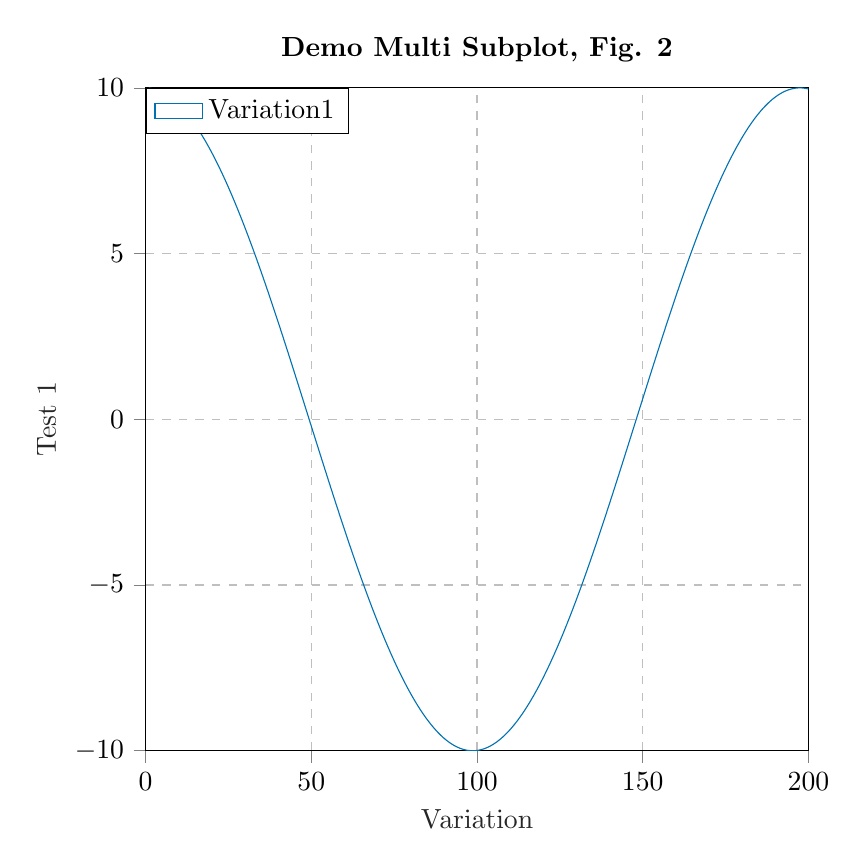
\begin{tikzpicture}

\begin{axis}[%
xmin=0,
xmax=200,
tick align=outside,
xlabel style={font=\color{white!15!black}},
xlabel={Variation},
ymin=-10,
ymax=10,
ylabel style={font=\color{white!15!black}},
ylabel={Test 1},
axis background/.style={fill=white},
title style={font=\bfseries},
title={Demo Multi Subplot, Fig. 2},
xmajorgrids,
xminorgrids,
ymajorgrids,
yminorgrids,
grid style={dashed},
x tick label style={/pgf/number format/.cd, fixed, fixed zerofill, precision=0, /tikz/.cd},
y tick label style={/pgf/number format/.cd, fixed, fixed zerofill, precision=0, /tikz/.cd},
xtick={0,50,100,150,200},
ytick={-10,-5,0,5,10},
ytick pos=left,
xtick pos=bottom,
/pgf/number format/.cd, set decimal separator={.},
/pgf/number format/.cd, 1000 sep={},
legend style={at={(0,1)}, anchor=north west},
legend cell align={left},
at={(0cm,0cm)},
height=10cm,
width=10cm
]
\addplot [color=mycolor1]
  table[row sep=crcr]{%
1	9.9949343685527\\
2	9.97974260633518\\
3	9.95444010452114\\
4	9.91905249774034\\
5	9.87361563810755\\
6	9.81817555889976\\
7	9.75278842791871\\
8	9.67752049058579\\
9	9.59244800282706\\
10	9.49765715381639\\
11	9.3932439786549\\
12	9.27931426107532\\
13	9.15598342626967\\
14	9.02337642394901\\
15	8.88162760175355\\
16	8.73088056914156\\
17	8.57128805189482\\
18	8.40301173738817\\
19	8.22622211077973\\
20	8.04109828228792\\
21	7.84782780573018\\
22	7.6466064885073\\
23	7.43763819322575\\
24	7.22113463115915\\
25	6.99731514775799\\
26	6.766406500425\\
27	6.52864262878125\\
28	6.28426441765578\\
29	6.03351945303887\\
30	5.77666177124611\\
31	5.51395160154758\\
32	5.24565510252271\\
33	4.97204409240804\\
34	4.69339577371098\\
35	4.40999245236874\\
36	4.12212125173668\\
37	3.83007382169614\\
38	3.53414604317627\\
39	3.23463772838926\\
40	2.93185231708274\\
41	2.62609656911697\\
42	2.31768025367836\\
43	2.00691583544419\\
44	1.69411815801639\\
45	1.37960412494525\\
46	1.06369237866609\\
47	0.746702977674199\\
48	0.428957072265208\\
49	0.110776579169256\\
50	-0.20751614459131\\
51	-0.525598628290302\\
52	-0.84314861420127\\
53	-1.15984438408527\\
54	-1.47536508513206\\
55	-1.78939105502456\\
56	-2.10160414579709\\
57	-2.41168804615947\\
58	-2.71932860196031\\
59	-3.02421413446482\\
60	-3.32603575612475\\
61	-3.62448768352046\\
62	-3.91926754715817\\
63	-4.21007669780842\\
64	-4.49662050907548\\
65	-4.77860867589107\\
66	-5.05575550863007\\
67	-5.32778022255019\\
68	-5.59440722226238\\
69	-5.85536638094374\\
70	-6.11039331401015\\
71	-6.35922964697119\\
72	-6.60162327719617\\
73	-6.8373286293259\\
74	-7.06610690407158\\
75	-7.28772632014861\\
76	-7.50196234910031\\
77	-7.70859794277358\\
78	-7.90742375321615\\
79	-8.09823834477244\\
80	-8.28084839816332\\
81	-8.45506890634298\\
82	-8.62072336193442\\
83	-8.77764393605372\\
84	-8.92567164834188\\
85	-9.06465652803202\\
86	-9.19445776588867\\
87	-9.31494385686537\\
88	-9.42599273333583\\
89	-9.52749188876388\\
90	-9.61933849168681\\
91	-9.70143948989658\\
92	-9.77371170471354\\
93	-9.83608191525683\\
94	-9.8884869326265\\
95	-9.93087366392173\\
96	-9.96319916603073\\
97	-9.9854306891375\\
98	-9.99754570990151\\
99	-9.99953195427674\\
100	-9.99138740994679\\
101	-9.97312032836364\\
102	-9.94474921638787\\
103	-9.90630281753889\\
104	-9.8578200828741\\
105	-9.79935013152657\\
106	-9.73095220094118\\
107	-9.65269558685952\\
108	-9.56465957311465\\
109	-9.46693335130652\\
110	-9.35961593043962\\
111	-9.24281603661433\\
112	-9.1166520028737\\
113	-8.98125164931709\\
114	-8.8367521536023\\
115	-8.68329991196725\\
116	-8.52105039091212\\
117	-8.35016796969213\\
118	-8.17082577378064\\
119	-7.98320549947113\\
120	-7.78749722979594\\
121	-7.58389924194814\\
122	-7.3726178064017\\
123	-7.15386697793345\\
124	-6.92786837875856\\
125	-6.69485097399922\\
126	-6.4550508397141\\
127	-6.20871092372347\\
128	-5.95608079947235\\
129	-5.69741641318113\\
130	-5.43297982453972\\
131	-5.16303894120795\\
132	-4.88786724739134\\
133	-4.60774352676701\\
134	-4.32295158004061\\
135	-4.03377993742041\\
136	-3.74052156629971\\
137	-3.4434735744439\\
138	-3.14293690898276\\
139	-2.83921605151301\\
140	-2.53261870962001\\
141	-2.22345550513112\\
142	-1.91203965941653\\
143	-1.59868667605651\\
144	-1.28371402119635\\
145	-0.967440801913169\\
146	-0.650187442920082\\
147	-0.332275361935487\\
148	-0.0140266440463831\\
149	0.304236284604565\\
150	0.622190983477373\\
151	0.939515324307746\\
152	1.25588781746372\\
153	1.57098793765521\\
154	1.88449644866663\\
155	2.19609572678351\\
156	2.50547008258541\\
157	2.8123060807792\\
158	3.11629285774853\\
159	3.41712243649802\\
160	3.71449003867279\\
161	4.00809439333744\\
162	4.29763804220156\\
163	4.58282764098255\\
164	4.86337425660038\\
165	5.13899365990337\\
166	5.40940661362814\\
167	5.67433915530226\\
168	5.93352287480283\\
169	6.18669518628982\\
170	6.4335995942387\\
171	6.6739859533028\\
172	6.90761072174211\\
173	7.13423720816187\\
174	7.35363581131079\\
175	7.56558425269615\\
176	7.76986780177998\\
177	7.96627949352819\\
178	8.15462033809232\\
179	8.33469952241136\\
180	8.50633460352948\\
181	8.66935169343383\\
182	8.82358563522498\\
183	8.96888017044177\\
184	9.10508809737087\\
185	9.23207142018067\\
186	9.34970148872851\\
187	9.4578591288995\\
188	9.556434763345\\
189	9.64532852249823\\
190	9.72445034575484\\
191	9.79372007271561\\
192	9.8530675243991\\
193	9.90243257434178\\
194	9.94176520951379\\
195	9.9710255809884\\
196	9.99018404431402\\
197	9.9992211895478\\
198	9.99812786092032\\
199	9.98690516611156\\
200	9.96556447512865\\
};
\legend{Variation1, Variation2}%
\end{axis}
\end{tikzpicture}%
	\caption[Example 0: A simple second plot]
	{
		Another plot
	}
\end{figure}

\pagebreak
\lstinputlisting[caption={eeeee}, label=Beispiel2]{Beispiel2.m}

\begin{figure}[H]
	\centering
	% This file was created by matlab2tikz.%
%
\definecolor{mycolor1}{rgb}{0.00000,0.44700,0.74100}%
\definecolor{mycolor2}{rgb}{0.00000,0.44706,0.69804}%
\definecolor{mycolor3}{rgb}{0.00000,0.61961,0.45098}%
\definecolor{mycolor4}{rgb}{0.83529,0.36863,0.00000}%
\definecolor{mycolor5}{rgb}{0.90196,0.62353,0.00000}%
%
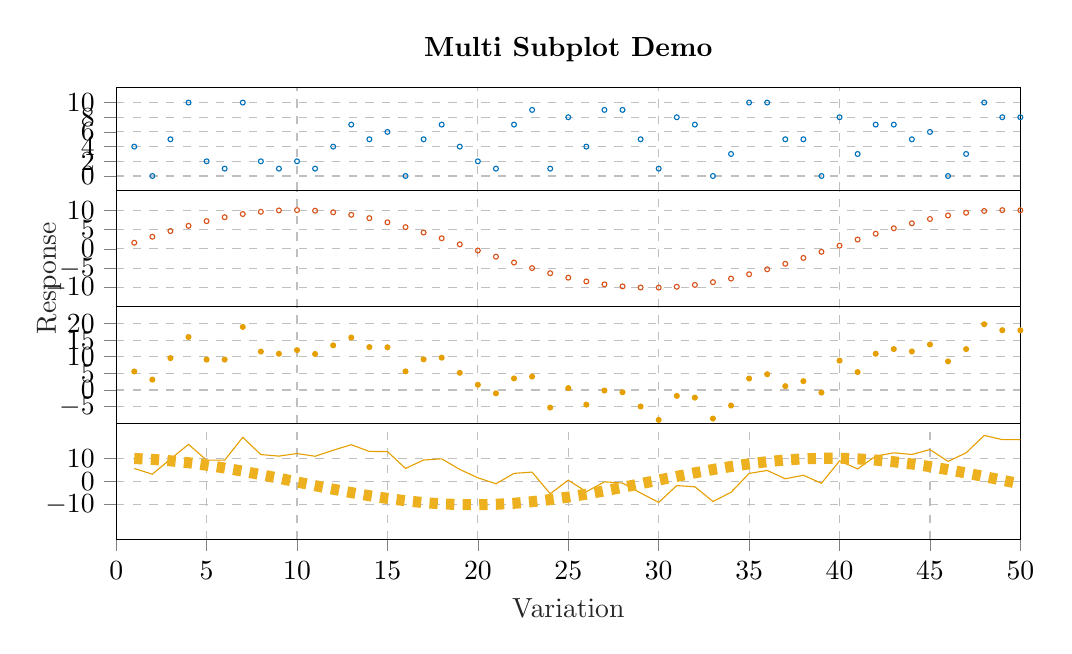
\begin{tikzpicture}

\begin{axis}[%
width=4.521in,
height=0.514in,
at={(0.758in,3.445in)},
scale only axis,
xmin=0,
xmax=50,
xtick={0,10,20,30,40,50},
xticklabels={\empty},
tick align=outside,
ymin=-2,
ymax=12,
ytick={ 0,  2,  4,  6,  8, 10},
axis background/.style={fill=white},
title style={font=\bfseries},
title={Multi Subplot Demo},
xmajorgrids,
xminorgrids,
ymajorgrids,
yminorgrids,
grid style={dashed},
x tick label style={/pgf/number format/.cd, fixed, fixed zerofill, precision=0, /tikz/.cd},
y tick label style={/pgf/number format/.cd, fixed, fixed zerofill, precision=0, /tikz/.cd},
ylabel style={at={(-0.05, 0.25)}},
ytick pos=left,
xtick pos=bottom,
/pgf/number format/.cd, set decimal separator={.},
/pgf/number format/.cd, 1000 sep={},
legend style={at={(0,1)}, anchor=north west},
legend cell align={left}
]
\addplot[only marks, mark=o, mark options={}, mark size=0.8839pt, draw=mycolor2] table[row sep=crcr]{%
x	y\\
1	4\\
2	0\\
3	5\\
4	10\\
5	2\\
6	1\\
7	10\\
8	2\\
9	1\\
10	2\\
11	1\\
12	4\\
13	7\\
14	5\\
15	6\\
16	0\\
17	5\\
18	7\\
19	4\\
20	2\\
21	1\\
22	7\\
23	9\\
24	1\\
25	8\\
26	4\\
27	9\\
28	9\\
29	5\\
30	1\\
31	8\\
32	7\\
33	0\\
34	3\\
35	10\\
36	10\\
37	5\\
38	5\\
39	0\\
40	8\\
41	3\\
42	7\\
43	7\\
44	5\\
45	6\\
46	0\\
47	3\\
48	10\\
49	8\\
50	8\\
};
\end{axis}

\begin{axis}[%
width=4.521in,
height=0.582in,
at={(0.758in,2.863in)},
scale only axis,
xmin=0,
xmax=50,
xtick={0,10,20,30,40,50},
xticklabels={\empty},
tick align=outside,
ymin=-15,
ymax=15,
ytick={-10,  -5,   0,   5,  10},
ylabel style={font=\color{white!15!black}},
ylabel={Response},
axis background/.style={fill=white},
xmajorgrids,
xminorgrids,
ymajorgrids,
yminorgrids,
grid style={dashed},
x tick label style={/pgf/number format/.cd, fixed, fixed zerofill, precision=0, /tikz/.cd},
y tick label style={/pgf/number format/.cd, fixed, fixed zerofill, precision=0, /tikz/.cd},
ylabel style={at={(-0.05, 0.25)}},
ytick pos=left,
xtick pos=bottom,
/pgf/number format/.cd, set decimal separator={.},
/pgf/number format/.cd, 1000 sep={},
legend style={at={(0,1)}, anchor=north west},
legend cell align={left}
]
\addplot[only marks, mark=o, mark options={}, mark size=0.8839pt, draw=mycolor3] table[row sep=crcr]{%
x	y\\
1	1.58483886591605\\
2	3.12961796207787\\
3	4.59529010441881\\
4	5.94480768524822\\
5	7.14405912090294\\
6	8.16273108589421\\
7	8.9750747389674\\
8	9.5605565732763\\
9	9.90437743921515\\
10	9.99784662063456\\
11	9.83860150896448\\
12	9.43066732256947\\
13	8.78435536181788\\
14	7.91600237165831\\
15	6.84755759980251\\
16	5.60602798839214\\
17	4.22279552296894\\
18	2.73282399403119\\
19	1.17377522176344\\
20	-0.414942916985869\\
21	-1.99317259657816\\
22	-3.52102110681844\\
23	-4.9598692158997\\
24	-6.27334734379666\\
25	-7.42825487149853\\
26	-8.39539934881863\\
27	-9.15033438823219\\
28	-9.67397759309389\\
29	-9.95309290094258\\
30	-9.98062514976289\\
31	-9.75587841041509\\
32	-9.28453357754716\\
33	-8.57850477434576\\
34	-7.65563820076495\\
35	-6.53926103740752\\
36	-5.2575918073579\\
37	-3.8430271001755\\
38	-2.33132268743488\\
39	-0.760689728650891\\
40	0.829171087323842\\
41	2.39807305154435\\
42	3.90635922928667\\
43	5.31590486332577\\
44	6.5910810485584\\
45	7.69965531929033\\
46	8.61360638515819\\
47	9.30983242170986\\
48	9.77073501227284\\
49	9.98466398088655\\
50	9.94621187231328\\
};
\end{axis}

\begin{axis}[%
width=4.521in,
height=0.582in,
at={(0.758in,2.282in)},
scale only axis,
xmin=0,
xmax=50,
xtick={0,10,20,30,40,50},
xticklabels={\empty},
tick align=outside,
ymin=-10,
ymax=25,
ytick={-5,  0,  5, 10, 15, 20},
axis background/.style={fill=white},
xmajorgrids,
xminorgrids,
ymajorgrids,
yminorgrids,
grid style={dashed},
x tick label style={/pgf/number format/.cd, fixed, fixed zerofill, precision=0, /tikz/.cd},
y tick label style={/pgf/number format/.cd, fixed, fixed zerofill, precision=0, /tikz/.cd},
ylabel style={at={(-0.05, 0.25)}},
ytick pos=left,
xtick pos=bottom,
/pgf/number format/.cd, set decimal separator={.},
/pgf/number format/.cd, 1000 sep={},
legend style={at={(0,1)}, anchor=north west},
legend cell align={left}
]
\addplot[only marks, mark=*, mark options={}, mark size=0.8839pt, color=mycolor4, fill=mycolor4] table[row sep=crcr]{%
x	y\\
1	5.58483886591605\\
2	3.12961796207787\\
3	9.59529010441881\\
4	15.9448076852482\\
5	9.14405912090294\\
6	9.16273108589421\\
7	18.9750747389674\\
8	11.5605565732763\\
9	10.9043774392151\\
10	11.9978466206346\\
11	10.8386015089645\\
12	13.4306673225695\\
13	15.7843553618179\\
14	12.9160023716583\\
15	12.8475575998025\\
16	5.60602798839214\\
17	9.22279552296894\\
18	9.73282399403119\\
19	5.17377522176344\\
20	1.58505708301413\\
21	-0.993172596578159\\
22	3.47897889318156\\
23	4.0401307841003\\
24	-5.27334734379666\\
25	0.571745128501471\\
26	-4.39539934881863\\
27	-0.15033438823219\\
28	-0.673977593093891\\
29	-4.95309290094258\\
30	-8.98062514976289\\
31	-1.75587841041509\\
32	-2.28453357754716\\
33	-8.57850477434576\\
34	-4.65563820076495\\
35	3.46073896259248\\
36	4.7424081926421\\
37	1.1569728998245\\
38	2.66867731256512\\
39	-0.760689728650891\\
40	8.82917108732384\\
41	5.39807305154435\\
42	10.9063592292867\\
43	12.3159048633258\\
44	11.5910810485584\\
45	13.6996553192903\\
46	8.61360638515819\\
47	12.3098324217099\\
48	19.7707350122728\\
49	17.9846639808865\\
50	17.9462118723133\\
};
\end{axis}

\begin{axis}[%
width=4.521in,
height=0.582in,
at={(0.758in,1.7in)},
scale only axis,
xmin=0,
xmax=50,
tick align=outside,
xlabel style={font=\color{white!15!black}},
xlabel={Variation},
ymin=-25,
ymax=25,
ytick={-10,   0,  10},
axis background/.style={fill=white},
xmajorgrids,
xminorgrids,
ymajorgrids,
yminorgrids,
grid style={dashed},
x tick label style={/pgf/number format/.cd, fixed, fixed zerofill, precision=0, /tikz/.cd},
y tick label style={/pgf/number format/.cd, fixed, fixed zerofill, precision=0, /tikz/.cd},
ylabel style={at={(-0.05, 0.25)}},
ytick pos=left,
xtick pos=bottom,
/pgf/number format/.cd, set decimal separator={.},
/pgf/number format/.cd, 1000 sep={},
legend style={at={(0,1)}, anchor=north west},
legend cell align={left}
]
\addplot [color=mycolor4, forget plot]
  table[row sep=crcr]{%
1	5.58483886591605\\
2	3.12961796207787\\
3	9.59529010441881\\
4	15.9448076852482\\
5	9.14405912090294\\
6	9.16273108589421\\
7	18.9750747389674\\
8	11.5605565732763\\
9	10.9043774392151\\
10	11.9978466206346\\
11	10.8386015089645\\
12	13.4306673225695\\
13	15.7843553618179\\
14	12.9160023716583\\
15	12.8475575998025\\
16	5.60602798839214\\
17	9.22279552296894\\
18	9.73282399403119\\
19	5.17377522176344\\
20	1.58505708301413\\
21	-0.993172596578159\\
22	3.47897889318156\\
23	4.0401307841003\\
24	-5.27334734379666\\
25	0.571745128501471\\
26	-4.39539934881863\\
27	-0.15033438823219\\
28	-0.673977593093891\\
29	-4.95309290094258\\
30	-8.98062514976289\\
31	-1.75587841041509\\
32	-2.28453357754716\\
33	-8.57850477434576\\
34	-4.65563820076495\\
35	3.46073896259248\\
36	4.7424081926421\\
37	1.1569728998245\\
38	2.66867731256512\\
39	-0.760689728650891\\
40	8.82917108732384\\
41	5.39807305154435\\
42	10.9063592292867\\
43	12.3159048633258\\
44	11.5910810485584\\
45	13.6996553192903\\
46	8.61360638515819\\
47	12.3098324217099\\
48	19.7707350122728\\
49	17.9846639808865\\
50	17.9462118723133\\
};
\addplot [color=mycolor5, dashed, line width=4.0pt, forget plot]
  table[row sep=crcr]{%
1	9.87361563810755\\
2	9.49765715381639\\
3	8.88162760175355\\
4	8.04109828228792\\
5	6.99731514775799\\
6	5.77666177124611\\
7	4.40999245236874\\
8	2.93185231708274\\
9	1.37960412494525\\
10	-0.20751614459131\\
11	-1.78939105502456\\
12	-3.32603575612475\\
13	-4.77860867589107\\
14	-6.11039331401015\\
15	-7.28772632014861\\
16	-8.28084839816332\\
17	-9.06465652803202\\
18	-9.61933849168681\\
19	-9.93087366392173\\
20	-9.99138740994679\\
21	-9.79935013152657\\
22	-9.35961593043962\\
23	-8.68329991196725\\
24	-7.78749722979594\\
25	-6.69485097399922\\
26	-5.43297982453972\\
27	-4.03377993742041\\
28	-2.53261870962001\\
29	-0.967440801913169\\
30	0.622190983477373\\
31	2.19609572678351\\
32	3.71449003867279\\
33	5.13899365990337\\
34	6.4335995942387\\
35	7.56558425269615\\
36	8.50633460352948\\
37	9.23207142018067\\
38	9.72445034575484\\
39	9.9710255809884\\
40	9.96556447512865\\
41	9.70820506785146\\
42	9.20545260004998\\
43	8.47001508169079\\
44	7.52048207306781\\
45	6.38085479885918\\
46	5.0799394722341\\
47	3.65061916387891\\
48	2.12902262081588\\
49	0.553611044675569\\
50	-1.03579408718833\\
};
\end{axis}
\end{tikzpicture}%
	\caption[Example 1: Multi Subplot with a single ylabel]
	{
		This is an example of a Matlab subplot with a single ylabel.
	}
\end{figure}

\begin{figure}[H]
	\centering
	% This file was created by matlab2tikz.%
%
\definecolor{mycolor1}{rgb}{0.00000,0.44700,0.74100}%
\definecolor{mycolor2}{rgb}{0.00000,0.44706,0.69804}%
\definecolor{mycolor3}{rgb}{0.00000,0.61961,0.45098}%
\definecolor{mycolor4}{rgb}{0.83529,0.36863,0.00000}%
\definecolor{mycolor5}{rgb}{0.90196,0.62353,0.00000}%
%
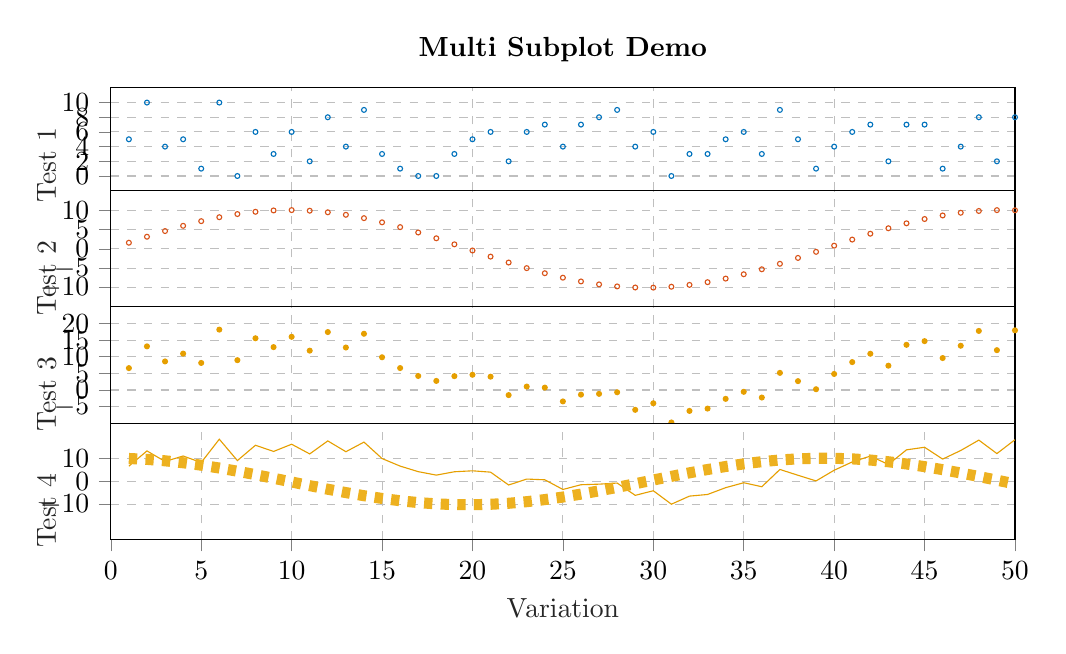
\begin{tikzpicture}

\begin{axis}[%
width=4.521in,
height=0.514in,
at={(0.758in,3.445in)},
scale only axis,
xmin=0,
xmax=50,
xtick={0,10,20,30,40,50},
xticklabels={\empty},
tick align=outside,
ymin=-2,
ymax=12,
ytick={ 0,  2,  4,  6,  8, 10},
ylabel style={font=\color{white!15!black}},
ylabel={Test 1},
axis background/.style={fill=white},
title style={font=\bfseries},
title={Multi Subplot Demo},
xmajorgrids,
xminorgrids,
ymajorgrids,
yminorgrids,
grid style={dashed},
x tick label style={/pgf/number format/.cd, fixed, fixed zerofill, precision=0, /tikz/.cd},
y tick label style={/pgf/number format/.cd, fixed, fixed zerofill, precision=0, /tikz/.cd},
ylabel style={at={(-0.05, 0.25)}},
ytick pos=left,
xtick pos=bottom,
/pgf/number format/.cd, set decimal separator={.},
/pgf/number format/.cd, 1000 sep={},
legend style={at={(0,1)}, anchor=north west},
legend cell align={left}
]
\addplot[only marks, mark=o, mark options={}, mark size=0.8839pt, draw=mycolor2] table[row sep=crcr]{%
x	y\\
1	5\\
2	10\\
3	4\\
4	5\\
5	1\\
6	10\\
7	0\\
8	6\\
9	3\\
10	6\\
11	2\\
12	8\\
13	4\\
14	9\\
15	3\\
16	1\\
17	0\\
18	0\\
19	3\\
20	5\\
21	6\\
22	2\\
23	6\\
24	7\\
25	4\\
26	7\\
27	8\\
28	9\\
29	4\\
30	6\\
31	0\\
32	3\\
33	3\\
34	5\\
35	6\\
36	3\\
37	9\\
38	5\\
39	1\\
40	4\\
41	6\\
42	7\\
43	2\\
44	7\\
45	7\\
46	1\\
47	4\\
48	8\\
49	2\\
50	8\\
};
\end{axis}

\begin{axis}[%
width=4.521in,
height=0.582in,
at={(0.758in,2.863in)},
scale only axis,
xmin=0,
xmax=50,
xtick={0,10,20,30,40,50},
xticklabels={\empty},
tick align=outside,
ymin=-15,
ymax=15,
ytick={-10,  -5,   0,   5,  10},
ylabel style={font=\color{white!15!black}},
ylabel={Test 2},
axis background/.style={fill=white},
xmajorgrids,
xminorgrids,
ymajorgrids,
yminorgrids,
grid style={dashed},
x tick label style={/pgf/number format/.cd, fixed, fixed zerofill, precision=0, /tikz/.cd},
y tick label style={/pgf/number format/.cd, fixed, fixed zerofill, precision=0, /tikz/.cd},
ylabel style={at={(-0.05, 0.25)}},
ytick pos=left,
xtick pos=bottom,
/pgf/number format/.cd, set decimal separator={.},
/pgf/number format/.cd, 1000 sep={},
legend style={at={(0,1)}, anchor=north west},
legend cell align={left}
]
\addplot[only marks, mark=o, mark options={}, mark size=0.8839pt, draw=mycolor3] table[row sep=crcr]{%
x	y\\
1	1.58483886591605\\
2	3.12961796207787\\
3	4.59529010441881\\
4	5.94480768524822\\
5	7.14405912090294\\
6	8.16273108589421\\
7	8.9750747389674\\
8	9.5605565732763\\
9	9.90437743921515\\
10	9.99784662063456\\
11	9.83860150896448\\
12	9.43066732256947\\
13	8.78435536181788\\
14	7.91600237165831\\
15	6.84755759980251\\
16	5.60602798839214\\
17	4.22279552296894\\
18	2.73282399403119\\
19	1.17377522176344\\
20	-0.414942916985869\\
21	-1.99317259657816\\
22	-3.52102110681844\\
23	-4.9598692158997\\
24	-6.27334734379666\\
25	-7.42825487149853\\
26	-8.39539934881863\\
27	-9.15033438823219\\
28	-9.67397759309389\\
29	-9.95309290094258\\
30	-9.98062514976289\\
31	-9.75587841041509\\
32	-9.28453357754716\\
33	-8.57850477434576\\
34	-7.65563820076495\\
35	-6.53926103740752\\
36	-5.2575918073579\\
37	-3.8430271001755\\
38	-2.33132268743488\\
39	-0.760689728650891\\
40	0.829171087323842\\
41	2.39807305154435\\
42	3.90635922928667\\
43	5.31590486332577\\
44	6.5910810485584\\
45	7.69965531929033\\
46	8.61360638515819\\
47	9.30983242170986\\
48	9.77073501227284\\
49	9.98466398088655\\
50	9.94621187231328\\
};
\end{axis}

\begin{axis}[%
width=4.521in,
height=0.582in,
at={(0.758in,2.282in)},
scale only axis,
xmin=0,
xmax=50,
xtick={0,10,20,30,40,50},
xticklabels={\empty},
tick align=outside,
ymin=-10,
ymax=25,
ytick={-5,  0,  5, 10, 15, 20},
ylabel style={font=\color{white!15!black}},
ylabel={Test 3},
axis background/.style={fill=white},
xmajorgrids,
xminorgrids,
ymajorgrids,
yminorgrids,
grid style={dashed},
x tick label style={/pgf/number format/.cd, fixed, fixed zerofill, precision=0, /tikz/.cd},
y tick label style={/pgf/number format/.cd, fixed, fixed zerofill, precision=0, /tikz/.cd},
ylabel style={at={(-0.05, 0.25)}},
ytick pos=left,
xtick pos=bottom,
/pgf/number format/.cd, set decimal separator={.},
/pgf/number format/.cd, 1000 sep={},
legend style={at={(0,1)}, anchor=north west},
legend cell align={left}
]
\addplot[only marks, mark=*, mark options={}, mark size=0.8839pt, color=mycolor4, fill=mycolor4] table[row sep=crcr]{%
x	y\\
1	6.58483886591605\\
2	13.1296179620779\\
3	8.59529010441881\\
4	10.9448076852482\\
5	8.14405912090294\\
6	18.1627310858942\\
7	8.9750747389674\\
8	15.5605565732763\\
9	12.9043774392151\\
10	15.9978466206346\\
11	11.8386015089645\\
12	17.4306673225695\\
13	12.7843553618179\\
14	16.9160023716583\\
15	9.84755759980251\\
16	6.60602798839214\\
17	4.22279552296894\\
18	2.73282399403119\\
19	4.17377522176344\\
20	4.58505708301413\\
21	4.00682740342184\\
22	-1.52102110681844\\
23	1.0401307841003\\
24	0.726652656203341\\
25	-3.42825487149853\\
26	-1.39539934881863\\
27	-1.15033438823219\\
28	-0.673977593093891\\
29	-5.95309290094258\\
30	-3.98062514976289\\
31	-9.75587841041509\\
32	-6.28453357754716\\
33	-5.57850477434576\\
34	-2.65563820076495\\
35	-0.539261037407515\\
36	-2.2575918073579\\
37	5.1569728998245\\
38	2.66867731256512\\
39	0.239310271349109\\
40	4.82917108732384\\
41	8.39807305154435\\
42	10.9063592292867\\
43	7.31590486332577\\
44	13.5910810485584\\
45	14.6996553192903\\
46	9.61360638515819\\
47	13.3098324217099\\
48	17.7707350122728\\
49	11.9846639808865\\
50	17.9462118723133\\
};
\end{axis}

\begin{axis}[%
width=4.521in,
height=0.582in,
at={(0.758in,1.7in)},
scale only axis,
xmin=0,
xmax=50,
tick align=outside,
xlabel style={font=\color{white!15!black}},
xlabel={Variation},
ymin=-25,
ymax=25,
ytick={-10,   0,  10},
ylabel style={font=\color{white!15!black}},
ylabel={Test 4},
axis background/.style={fill=white},
xmajorgrids,
xminorgrids,
ymajorgrids,
yminorgrids,
grid style={dashed},
x tick label style={/pgf/number format/.cd, fixed, fixed zerofill, precision=0, /tikz/.cd},
y tick label style={/pgf/number format/.cd, fixed, fixed zerofill, precision=0, /tikz/.cd},
ylabel style={at={(-0.05, 0.25)}},
ytick pos=left,
xtick pos=bottom,
/pgf/number format/.cd, set decimal separator={.},
/pgf/number format/.cd, 1000 sep={},
legend style={at={(0,1)}, anchor=north west},
legend cell align={left}
]
\addplot [color=mycolor4, forget plot]
  table[row sep=crcr]{%
1	6.58483886591605\\
2	13.1296179620779\\
3	8.59529010441881\\
4	10.9448076852482\\
5	8.14405912090294\\
6	18.1627310858942\\
7	8.9750747389674\\
8	15.5605565732763\\
9	12.9043774392151\\
10	15.9978466206346\\
11	11.8386015089645\\
12	17.4306673225695\\
13	12.7843553618179\\
14	16.9160023716583\\
15	9.84755759980251\\
16	6.60602798839214\\
17	4.22279552296894\\
18	2.73282399403119\\
19	4.17377522176344\\
20	4.58505708301413\\
21	4.00682740342184\\
22	-1.52102110681844\\
23	1.0401307841003\\
24	0.726652656203341\\
25	-3.42825487149853\\
26	-1.39539934881863\\
27	-1.15033438823219\\
28	-0.673977593093891\\
29	-5.95309290094258\\
30	-3.98062514976289\\
31	-9.75587841041509\\
32	-6.28453357754716\\
33	-5.57850477434576\\
34	-2.65563820076495\\
35	-0.539261037407515\\
36	-2.2575918073579\\
37	5.1569728998245\\
38	2.66867731256512\\
39	0.239310271349109\\
40	4.82917108732384\\
41	8.39807305154435\\
42	10.9063592292867\\
43	7.31590486332577\\
44	13.5910810485584\\
45	14.6996553192903\\
46	9.61360638515819\\
47	13.3098324217099\\
48	17.7707350122728\\
49	11.9846639808865\\
50	17.9462118723133\\
};
\addplot [color=mycolor5, dashed, line width=4.0pt, forget plot]
  table[row sep=crcr]{%
1	9.87361563810755\\
2	9.49765715381639\\
3	8.88162760175355\\
4	8.04109828228792\\
5	6.99731514775799\\
6	5.77666177124611\\
7	4.40999245236874\\
8	2.93185231708274\\
9	1.37960412494525\\
10	-0.20751614459131\\
11	-1.78939105502456\\
12	-3.32603575612475\\
13	-4.77860867589107\\
14	-6.11039331401015\\
15	-7.28772632014861\\
16	-8.28084839816332\\
17	-9.06465652803202\\
18	-9.61933849168681\\
19	-9.93087366392173\\
20	-9.99138740994679\\
21	-9.79935013152657\\
22	-9.35961593043962\\
23	-8.68329991196725\\
24	-7.78749722979594\\
25	-6.69485097399922\\
26	-5.43297982453972\\
27	-4.03377993742041\\
28	-2.53261870962001\\
29	-0.967440801913169\\
30	0.622190983477373\\
31	2.19609572678351\\
32	3.71449003867279\\
33	5.13899365990337\\
34	6.4335995942387\\
35	7.56558425269615\\
36	8.50633460352948\\
37	9.23207142018067\\
38	9.72445034575484\\
39	9.9710255809884\\
40	9.96556447512865\\
41	9.70820506785146\\
42	9.20545260004998\\
43	8.47001508169079\\
44	7.52048207306781\\
45	6.38085479885918\\
46	5.0799394722341\\
47	3.65061916387891\\
48	2.12902262081588\\
49	0.553611044675569\\
50	-1.03579408718833\\
};
\end{axis}
\end{tikzpicture}%
	\caption[Example 1: Multi Subplot with a ylabel for each plot]
	{
		This is an example of a Matlab subplot with a ylabel for each plot.
	}
\end{figure}

\lipsum[1-4]

\begin{figure}[H]
	\centering
	% This file was created by matlab2tikz.%
%
\definecolor{mycolor1}{rgb}{0.90196,0.62353,0.00000}%
\definecolor{mycolor2}{rgb}{0.00000,0.61961,0.45098}%
\definecolor{mycolor3}{rgb}{0.00000,0.44706,0.69804}%
\definecolor{mycolor4}{rgb}{0.19608,0.19608,0.19608}%
%
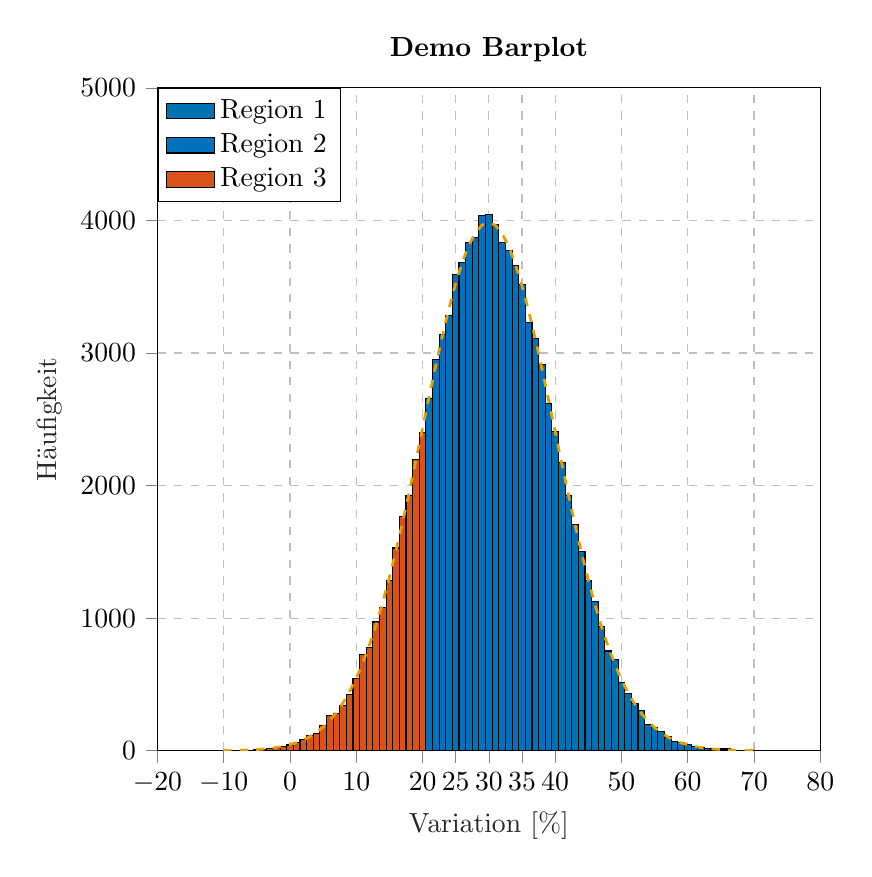
\begin{tikzpicture} 
\pgfplotsset{legend image code/.code={\draw [#1] (0cm,-0.1cm) rectangle (0.6cm,0.1cm);},}

\begin{axis}[%
%bar shift auto,
xmin=-20,
xmax=80,
xtick={-20, -10,   0,  10,  20,  25,  30,  35,  40,  50,  60,  70,  80},
tick align=outside,
xlabel style={font=\color{white!15!black}},
xlabel={Variation [\%]},
ymin=0,
ymax=5000,
ylabel style={font=\color{white!15!black}},
ylabel={Häufigkeit},
axis background/.style={fill=white},
title style={font=\bfseries},
title={Demo Barplot},
xmajorgrids,
xminorgrids,
ymajorgrids,
yminorgrids,
grid style={dashed},
x tick label style={/pgf/number format/.cd, fixed, fixed zerofill, precision=0, /tikz/.cd},
y tick label style={/pgf/number format/.cd, fixed, fixed zerofill, precision=0, /tikz/.cd},
xtick={-20,-10,0,10,20,25,30,35,40,50,60,70,80},
ytick={0,1000,2000,3000,4000,5000},
ytick pos=left,
xtick pos=bottom,
/pgf/number format/.cd, set decimal separator={.},
/pgf/number format/.cd, 1000 sep={},
legend style={at={(0,1)}, anchor=north west},
legend cell align={left},
at={(0cm,0cm)},
height=10cm,
width=10cm
]
\addplot[ybar, bar width=1, fill=mycolor1, draw=black] table[row sep=crcr] {%
40	2409\\
41	2174\\
42	1922\\
43	1704\\
44	1505\\
45	1281\\
46	1128\\
47	935\\
48	752\\
49	688\\
50	513\\
51	432\\
52	356\\
53	306\\
54	199\\
55	172\\
56	142\\
57	104\\
58	73\\
59	61\\
60	44\\
61	31\\
62	25\\
63	18\\
64	14\\
65	13\\
66	13\\
67	4\\
68	4\\
69	1\\
70	3\\
};
\addplot [color=black, forget plot]
  table[row sep=crcr]{%
-20	0\\
80	0\\
};
\addplot[ybar, bar width=1, fill=mycolor2, draw=black] table[row sep=crcr] {%
21	2658\\
22	2952\\
23	3142\\
24	3280\\
25	3589\\
26	3686\\
27	3834\\
28	3872\\
29	4040\\
30	4046\\
31	3968\\
32	3834\\
33	3774\\
34	3663\\
35	3519\\
36	3230\\
37	3110\\
38	2913\\
39	2619\\
};
\addplot [color=black, forget plot]
  table[row sep=crcr]{%
-20	0\\
80	0\\
};
\addplot[ybar, bar width=1, fill=mycolor3, draw=black] table[row sep=crcr] {%
-10	2\\
-9	1\\
-8	3\\
-7	5\\
-6	1\\
-5	12\\
-4	9\\
-3	14\\
-2	21\\
-1	29\\
0	43\\
1	64\\
2	85\\
3	112\\
4	130\\
5	189\\
6	265\\
7	283\\
8	344\\
9	424\\
10	544\\
11	727\\
12	776\\
13	971\\
14	1083\\
15	1285\\
16	1529\\
17	1769\\
18	1922\\
19	2200\\
20	2403\\
};
\addplot [color=black, forget plot]
  table[row sep=crcr]{%
-20	0\\
80	0\\
};
\addplot [color=mycolor4, dashed, line width=1.0pt, forget plot]
  table[row sep=crcr]{%
-10.1089970806553	1.33646787696355\\
-9.10762452190028	1.98383178823833\\
-8.10625196314528	2.91546760732525\\
-7.10487940439028	4.24198033825572\\
-6.10350684563528	6.11063209955091\\
-5.10213428688028	8.71486528581093\\
-4.10076172812529	12.3053019348266\\
-3.09938916937029	17.2020785270503\\
-2.09801661061529	23.8082038560051\\
-1.09664405186029	32.6234130108532\\
-0.0952714931052938	44.2577377739221\\
0.906101065649706	59.44373417998\\
1.9074736244047	79.0460205222841\\
2.9088461831597	104.066510743802\\
3.9102187419147	135.643513644645\\
4.9115913006697	175.042748478762\\
5.9129638594247	223.638346178429\\
6.91433641817969	282.882105106016\\
7.91570897693469	354.259686228439\\
8.91708153568969	439.233086585794\\
9.91845409444469	539.169623145204\\
10.9198266531997	655.258766589894\\
11.9211992119547	788.41943101629\\
12.9225717707097	939.201664301824\\
13.9239443294647	1107.68797995986\\
14.9253168882197	1293.40068822058\\
15.9266894469747	1495.22237579488\\
16.9280620057297	1711.33700988241\\
17.9294345644847	1939.19888542426\\
18.9308071232397	2175.53571972658\\
19.9321796819947	2416.39060710815\\
20.9335522407497	2657.20532855002\\
21.9349247995047	2892.94479091433\\
22.9362973582597	3118.25933951081\\
23.9376699170147	3327.67859452926\\
24.9390424757697	3515.82758770643\\
25.9404150345247	3677.65360737658\\
26.9417875932797	3808.65055793722\\
27.9431601520347	3905.06700584683\\
28.9445327107897	3964.08453583491\\
29.9459052695446	3983.95459225921\\
30.9472778282997	3964.08453583491\\
31.9486503870547	3905.06700584683\\
32.9500229458096	3808.65055793722\\
33.9513955045646	3677.65360737658\\
34.9527680633196	3515.82758770643\\
35.9541406220746	3327.67859452925\\
36.9555131808296	3118.25933951081\\
37.9568857395846	2892.94479091433\\
38.9582582983396	2657.20532855002\\
39.9596308570946	2416.39060710815\\
40.9610034158496	2175.53571972658\\
41.9623759746046	1939.19888542426\\
42.9637485333596	1711.33700988241\\
43.9651210921146	1495.22237579488\\
44.9664936508696	1293.40068822058\\
45.9678662096246	1107.68797995985\\
46.9692387683796	939.201664301822\\
47.9706113271346	788.419431016289\\
48.9719838858896	655.258766589894\\
49.9733564446446	539.169623145203\\
50.9747290033996	439.233086585793\\
51.9761015621546	354.259686228439\\
52.9774741209096	282.882105106016\\
53.9788466796646	223.638346178428\\
54.9802192384196	175.042748478762\\
55.9815917971746	135.643513644644\\
56.9829643559296	104.066510743802\\
57.9843369146846	79.0460205222838\\
58.9857094734396	59.44373417998\\
59.9870820321946	44.2577377739219\\
60.9884545909496	32.6234130108531\\
61.9898271497046	23.8082038560051\\
62.9911997084596	17.2020785270503\\
63.9925722672146	12.3053019348266\\
64.9939448259696	8.71486528581092\\
65.9953173847246	6.11063209955091\\
66.9966899434796	4.2419803382557\\
67.9980625022346	2.91546760732525\\
68.9994350609896	1.98383178823833\\
70.0008076197446	1.33646787696355\\
};
\legend{Region 1, Region 2, Region 3}% 
\end{axis}%
\end{tikzpicture}%
	\caption[Example 2: Barplot]
	{
		A barplot with a special legend
	}
\end{figure}

\lipsum[1-5]

\pagebreak
\lstinputlisting[caption={eeeee}, label=Beispiel3]{Beispiel3.m}

\begin{figure}[H]
	\centering
	% This file was created by matlab2tikz.%
%
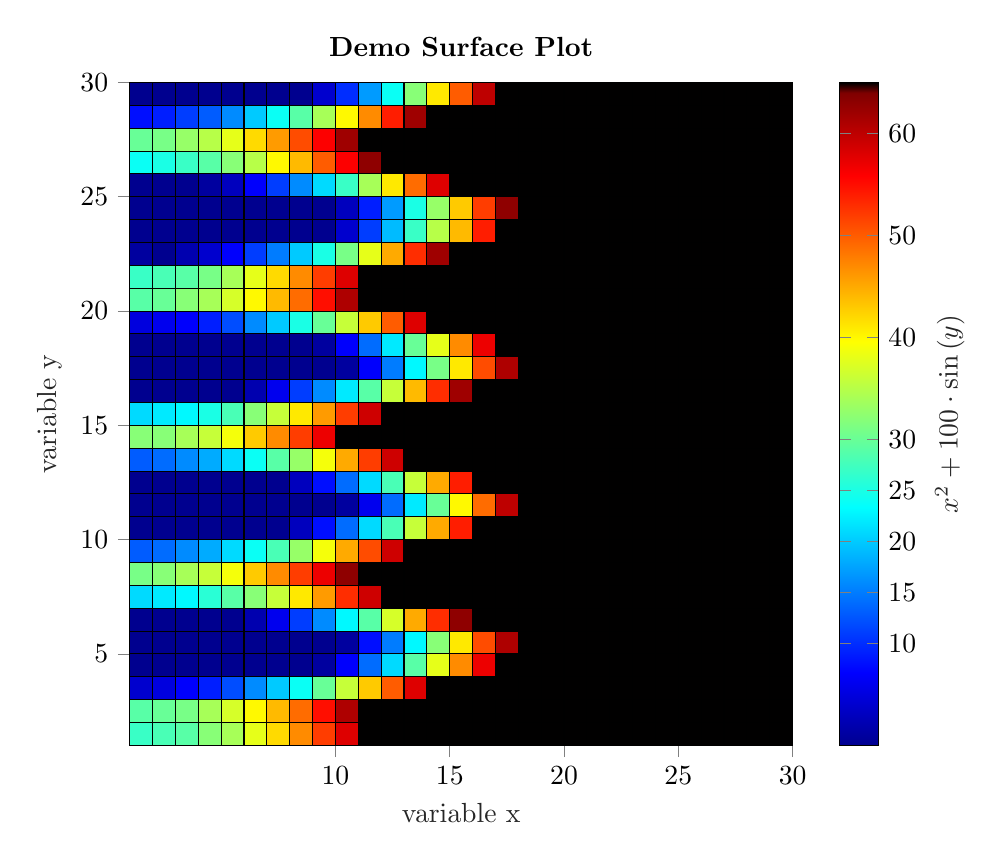
\begin{tikzpicture}

\begin{axis}[%
point meta min=0,
point meta max=65,
xmin=1,
xmax=30,
xtick={10, 15, 20, 25, 30},
tick align=outside,
xlabel style={font=\color{white!15!black}},
xlabel={variable x},
ymin=1,
ymax=30,
ylabel style={font=\color{white!15!black}},
ylabel={variable y},
axis background/.style={fill=white},
title style={font=\bfseries},
title={Demo Surface Plot},
xmajorgrids,
xminorgrids,
ymajorgrids,
yminorgrids,
grid style={dashed},
x tick label style={/pgf/number format/.cd, fixed, fixed zerofill, precision=0, /tikz/.cd},
y tick label style={/pgf/number format/.cd, fixed, fixed zerofill, precision=0, /tikz/.cd},
xtick={10,15,20,25,30},
ytick={5,10,15,20,25,30},
ytick pos=left,
xtick pos=bottom,
/pgf/number format/.cd, set decimal separator={.},
/pgf/number format/.cd, 1000 sep={},
legend style={at={(0,1)}, anchor=north west},
legend cell align={left},
at={(0cm,0cm)},
height=10cm,
width=10cm,
colorbar style={ytick={10,15,20,25,30,40,50,60,70}},
colormap={mymap}{[1pt] rgb(0pt)=(0,0,0.5625); rgb(7pt)=(0,0,1); rgb(23pt)=(0,1,1); rgb(39pt)=(1,1,0); rgb(55pt)=(1,0,0); rgb(63pt)=(0.5,0,0); rgb(64pt)=(0,0,0)},
colorbar,
colorbar style={ylabel style={font=\color{white!15!black}}, ylabel={$x^{2}+100\cdot\sin\left(y\right)$}}
]

\addplot[%
surf,
shader=flat corner, draw=black, colormap={mymap}{[1pt] rgb(0pt)=(0,0,0.5625); rgb(7pt)=(0,0,1); rgb(23pt)=(0,1,1); rgb(39pt)=(1,1,0); rgb(55pt)=(1,0,0); rgb(63pt)=(0.5,0,0); rgb(64pt)=(0,0,0)}, mesh/rows=30]
table[row sep=crcr, point meta=\thisrow{c}] {%
%
x	y	c\\
1	1	27\\
1	2	29\\
1	3	4\\
1	4	0\\
1	5	0\\
1	6	0\\
1	7	21\\
1	8	31\\
1	9	13\\
1	10	0\\
1	11	0\\
1	12	0\\
1	13	13\\
1	14	32\\
1	15	21\\
1	16	0\\
1	17	0\\
1	18	0\\
1	19	5\\
1	20	29\\
1	21	27\\
1	22	1\\
1	23	0\\
1	24	0\\
1	25	0\\
1	26	24\\
1	27	30\\
1	28	8\\
1	29	0\\
1	30	0\\
2	1	28\\
2	2	30\\
2	3	5\\
2	4	0\\
2	5	0\\
2	6	0\\
2	7	22\\
2	8	32\\
2	9	14\\
2	10	0\\
2	11	0\\
2	12	0\\
2	13	14\\
2	14	32\\
2	15	22\\
2	16	0\\
2	17	0\\
2	18	0\\
2	19	6\\
2	20	30\\
2	21	28\\
2	22	0\\
2	23	0\\
2	24	0\\
2	25	0\\
2	26	25\\
2	27	31\\
2	28	9\\
2	29	0\\
2	30	0\\
3	1	29\\
3	2	31\\
3	3	7\\
3	4	0\\
3	5	0\\
3	6	0\\
3	7	23\\
3	8	34\\
3	9	16\\
3	10	0\\
3	11	0\\
3	12	0\\
3	13	16\\
3	14	34\\
3	15	23\\
3	16	0\\
3	17	0\\
3	18	0\\
3	19	7\\
3	20	32\\
3	21	29\\
3	22	2\\
3	23	0\\
3	24	0\\
3	25	0\\
3	26	27\\
3	27	33\\
3	28	11\\
3	29	0\\
3	30	0\\
4	1	32\\
4	2	34\\
4	3	9\\
4	4	0\\
4	5	0\\
4	6	0\\
4	7	26\\
4	8	36\\
4	9	18\\
4	10	0\\
4	11	0\\
4	12	0\\
4	13	18\\
4	14	36\\
4	15	25\\
4	16	0\\
4	17	0\\
4	18	0\\
4	19	9\\
4	20	34\\
4	21	31\\
4	22	4\\
4	23	0\\
4	24	0\\
4	25	1\\
4	26	29\\
4	27	35\\
4	28	13\\
4	29	0\\
4	30	0\\
5	1	34\\
5	2	37\\
5	3	12\\
5	4	0\\
5	5	0\\
5	6	0\\
5	7	29\\
5	8	39\\
5	9	21\\
5	10	0\\
5	11	0\\
5	12	0\\
5	13	21\\
5	14	39\\
5	15	28\\
5	16	0\\
5	17	0\\
5	18	0\\
5	19	12\\
5	20	37\\
5	21	34\\
5	22	7\\
5	23	0\\
5	24	0\\
5	25	3\\
5	26	32\\
5	27	38\\
5	28	16\\
5	29	0\\
5	30	0\\
6	1	38\\
6	2	40\\
6	3	16\\
6	4	0\\
6	5	0\\
6	6	2\\
6	7	32\\
6	8	43\\
6	9	24\\
6	10	0\\
6	11	0\\
6	12	0\\
6	13	24\\
6	14	43\\
6	15	32\\
6	16	2\\
6	17	0\\
6	18	0\\
6	19	16\\
6	20	40\\
6	21	38\\
6	22	11\\
6	23	0\\
6	24	0\\
6	25	7\\
6	26	35\\
6	27	42\\
6	28	20\\
6	29	0\\
6	30	0\\
7	1	42\\
7	2	44\\
7	3	20\\
7	4	0\\
7	5	0\\
7	6	6\\
7	7	36\\
7	8	47\\
7	9	28\\
7	10	0\\
7	11	0\\
7	12	0\\
7	13	29\\
7	14	47\\
7	15	36\\
7	16	6\\
7	17	0\\
7	18	0\\
7	19	20\\
7	20	44\\
7	21	42\\
7	22	15\\
7	23	0\\
7	24	0\\
7	25	11\\
7	26	40\\
7	27	46\\
7	28	24\\
7	29	0\\
7	30	0\\
8	1	47\\
8	2	49\\
8	3	24\\
8	4	0\\
8	5	0\\
8	6	11\\
8	7	41\\
8	8	52\\
8	9	33\\
8	10	3\\
8	11	0\\
8	12	3\\
8	13	33\\
8	14	52\\
8	15	41\\
8	16	11\\
8	17	0\\
8	18	0\\
8	19	25\\
8	20	49\\
8	21	47\\
8	22	20\\
8	23	0\\
8	24	0\\
8	25	16\\
8	26	44\\
8	27	51\\
8	28	29\\
8	29	0\\
8	30	0\\
9	1	52\\
9	2	55\\
9	3	30\\
9	4	1\\
9	5	0\\
9	6	16\\
9	7	46\\
9	8	57\\
9	9	39\\
9	10	8\\
9	11	0\\
9	12	8\\
9	13	39\\
9	14	57\\
9	15	46\\
9	16	16\\
9	17	0\\
9	18	1\\
9	19	30\\
9	20	55\\
9	21	52\\
9	22	25\\
9	23	0\\
9	24	0\\
9	25	21\\
9	26	50\\
9	27	56\\
9	28	34\\
9	29	4\\
9	30	0\\
10	1	58\\
10	2	61\\
10	3	36\\
10	4	7\\
10	5	1\\
10	6	23\\
10	7	53\\
10	8	63\\
10	9	45\\
10	10	14\\
10	11	1\\
10	12	14\\
10	13	45\\
10	14	65\\
10	15	52\\
10	16	22\\
10	17	1\\
10	18	7\\
10	19	36\\
10	20	61\\
10	21	58\\
10	22	31\\
10	23	4\\
10	24	3\\
10	25	27\\
10	26	56\\
10	27	62\\
10	28	40\\
10	29	10\\
10	30	1\\
11	1	65\\
11	2	65\\
11	3	43\\
11	4	14\\
11	5	8\\
11	6	29\\
11	7	59\\
11	8	65\\
11	9	51\\
11	10	21\\
11	11	6\\
11	12	21\\
11	13	52\\
11	14	65\\
11	15	59\\
11	16	29\\
11	17	7\\
11	18	14\\
11	19	43\\
11	20	65\\
11	21	65\\
11	22	38\\
11	23	11\\
11	24	9\\
11	25	34\\
11	26	63\\
11	27	65\\
11	28	47\\
11	29	17\\
11	30	7\\
12	1	65\\
12	2	65\\
12	3	50\\
12	4	21\\
12	5	15\\
12	6	37\\
12	7	65\\
12	8	65\\
12	9	59\\
12	10	28\\
12	11	14\\
12	12	28\\
12	13	59\\
12	14	65\\
12	15	65\\
12	16	36\\
12	17	15\\
12	18	22\\
12	19	50\\
12	20	65\\
12	21	65\\
12	22	45\\
12	23	19\\
12	24	17\\
12	25	41\\
12	26	65\\
12	27	65\\
12	28	54\\
12	29	24\\
12	30	14\\
13	1	65\\
13	2	65\\
13	3	58\\
13	4	29\\
13	5	23\\
13	6	45\\
13	7	65\\
13	8	65\\
13	9	65\\
13	10	36\\
13	11	22\\
13	12	36\\
13	13	65\\
13	14	65\\
13	15	65\\
13	16	44\\
13	17	23\\
13	18	30\\
13	19	58\\
13	20	65\\
13	21	65\\
13	22	53\\
13	23	27\\
13	24	25\\
13	25	49\\
13	26	65\\
13	27	65\\
13	28	62\\
13	29	32\\
13	30	22\\
14	1	65\\
14	2	65\\
14	3	65\\
14	4	38\\
14	5	32\\
14	6	53\\
14	7	65\\
14	8	65\\
14	9	65\\
14	10	45\\
14	11	30\\
14	12	45\\
14	13	65\\
14	14	65\\
14	15	65\\
14	16	53\\
14	17	31\\
14	18	38\\
14	19	65\\
14	20	65\\
14	21	65\\
14	22	62\\
14	23	35\\
14	24	33\\
14	25	58\\
14	26	65\\
14	27	65\\
14	28	65\\
14	29	41\\
14	30	31\\
15	1	65\\
15	2	65\\
15	3	65\\
15	4	47\\
15	5	41\\
15	6	63\\
15	7	65\\
15	8	65\\
15	9	65\\
15	10	54\\
15	11	40\\
15	12	54\\
15	13	65\\
15	14	65\\
15	15	65\\
15	16	62\\
15	17	41\\
15	18	47\\
15	19	65\\
15	20	65\\
15	21	65\\
15	22	65\\
15	23	44\\
15	24	43\\
15	25	65\\
15	26	65\\
15	27	65\\
15	28	65\\
15	29	50\\
15	30	40\\
16	1	65\\
16	2	65\\
16	3	65\\
16	4	57\\
16	5	51\\
16	6	65\\
16	7	65\\
16	8	65\\
16	9	65\\
16	10	65\\
16	11	49\\
16	12	65\\
16	13	65\\
16	14	65\\
16	15	65\\
16	16	65\\
16	17	51\\
16	18	57\\
16	19	65\\
16	20	65\\
16	21	65\\
16	22	65\\
16	23	54\\
16	24	52\\
16	25	65\\
16	26	65\\
16	27	65\\
16	28	65\\
16	29	60\\
16	30	50\\
17	1	65\\
17	2	65\\
17	3	65\\
17	4	65\\
17	5	61\\
17	6	65\\
17	7	65\\
17	8	65\\
17	9	65\\
17	10	65\\
17	11	60\\
17	12	65\\
17	13	65\\
17	14	65\\
17	15	65\\
17	16	65\\
17	17	61\\
17	18	65\\
17	19	65\\
17	20	65\\
17	21	65\\
17	22	65\\
17	23	65\\
17	24	63\\
17	25	65\\
17	26	65\\
17	27	65\\
17	28	65\\
17	29	65\\
17	30	60\\
18	1	65\\
18	2	65\\
18	3	65\\
18	4	65\\
18	5	65\\
18	6	65\\
18	7	65\\
18	8	65\\
18	9	65\\
18	10	65\\
18	11	65\\
18	12	65\\
18	13	65\\
18	14	65\\
18	15	65\\
18	16	65\\
18	17	65\\
18	18	65\\
18	19	65\\
18	20	65\\
18	21	65\\
18	22	65\\
18	23	65\\
18	24	65\\
18	25	65\\
18	26	65\\
18	27	65\\
18	28	65\\
18	29	65\\
18	30	65\\
19	1	65\\
19	2	65\\
19	3	65\\
19	4	65\\
19	5	65\\
19	6	65\\
19	7	65\\
19	8	65\\
19	9	65\\
19	10	65\\
19	11	65\\
19	12	65\\
19	13	65\\
19	14	65\\
19	15	65\\
19	16	65\\
19	17	65\\
19	18	65\\
19	19	65\\
19	20	65\\
19	21	65\\
19	22	65\\
19	23	65\\
19	24	65\\
19	25	65\\
19	26	65\\
19	27	65\\
19	28	65\\
19	29	65\\
19	30	65\\
20	1	65\\
20	2	65\\
20	3	65\\
20	4	65\\
20	5	65\\
20	6	65\\
20	7	65\\
20	8	65\\
20	9	65\\
20	10	65\\
20	11	65\\
20	12	65\\
20	13	65\\
20	14	65\\
20	15	65\\
20	16	65\\
20	17	65\\
20	18	65\\
20	19	65\\
20	20	65\\
20	21	65\\
20	22	65\\
20	23	65\\
20	24	65\\
20	25	65\\
20	26	65\\
20	27	65\\
20	28	65\\
20	29	65\\
20	30	65\\
21	1	65\\
21	2	65\\
21	3	65\\
21	4	65\\
21	5	65\\
21	6	65\\
21	7	65\\
21	8	65\\
21	9	65\\
21	10	65\\
21	11	65\\
21	12	65\\
21	13	65\\
21	14	65\\
21	15	65\\
21	16	65\\
21	17	65\\
21	18	65\\
21	19	65\\
21	20	65\\
21	21	65\\
21	22	65\\
21	23	65\\
21	24	65\\
21	25	65\\
21	26	65\\
21	27	65\\
21	28	65\\
21	29	65\\
21	30	65\\
22	1	65\\
22	2	65\\
22	3	65\\
22	4	65\\
22	5	65\\
22	6	65\\
22	7	65\\
22	8	65\\
22	9	65\\
22	10	65\\
22	11	65\\
22	12	65\\
22	13	65\\
22	14	65\\
22	15	65\\
22	16	65\\
22	17	65\\
22	18	65\\
22	19	65\\
22	20	65\\
22	21	65\\
22	22	65\\
22	23	65\\
22	24	65\\
22	25	65\\
22	26	65\\
22	27	65\\
22	28	65\\
22	29	65\\
22	30	65\\
23	1	65\\
23	2	65\\
23	3	65\\
23	4	65\\
23	5	65\\
23	6	65\\
23	7	65\\
23	8	65\\
23	9	65\\
23	10	65\\
23	11	65\\
23	12	65\\
23	13	65\\
23	14	65\\
23	15	65\\
23	16	65\\
23	17	65\\
23	18	65\\
23	19	65\\
23	20	65\\
23	21	65\\
23	22	65\\
23	23	65\\
23	24	65\\
23	25	65\\
23	26	65\\
23	27	65\\
23	28	65\\
23	29	65\\
23	30	65\\
24	1	65\\
24	2	65\\
24	3	65\\
24	4	65\\
24	5	65\\
24	6	65\\
24	7	65\\
24	8	65\\
24	9	65\\
24	10	65\\
24	11	65\\
24	12	65\\
24	13	65\\
24	14	65\\
24	15	65\\
24	16	65\\
24	17	65\\
24	18	65\\
24	19	65\\
24	20	65\\
24	21	65\\
24	22	65\\
24	23	65\\
24	24	65\\
24	25	65\\
24	26	65\\
24	27	65\\
24	28	65\\
24	29	65\\
24	30	65\\
25	1	65\\
25	2	65\\
25	3	65\\
25	4	65\\
25	5	65\\
25	6	65\\
25	7	65\\
25	8	65\\
25	9	65\\
25	10	65\\
25	11	65\\
25	12	65\\
25	13	65\\
25	14	65\\
25	15	65\\
25	16	65\\
25	17	65\\
25	18	65\\
25	19	65\\
25	20	65\\
25	21	65\\
25	22	65\\
25	23	65\\
25	24	65\\
25	25	65\\
25	26	65\\
25	27	65\\
25	28	65\\
25	29	65\\
25	30	65\\
26	1	65\\
26	2	65\\
26	3	65\\
26	4	65\\
26	5	65\\
26	6	65\\
26	7	65\\
26	8	65\\
26	9	65\\
26	10	65\\
26	11	65\\
26	12	65\\
26	13	65\\
26	14	65\\
26	15	65\\
26	16	65\\
26	17	65\\
26	18	65\\
26	19	65\\
26	20	65\\
26	21	65\\
26	22	65\\
26	23	65\\
26	24	65\\
26	25	65\\
26	26	65\\
26	27	65\\
26	28	65\\
26	29	65\\
26	30	65\\
27	1	65\\
27	2	65\\
27	3	65\\
27	4	65\\
27	5	65\\
27	6	65\\
27	7	65\\
27	8	65\\
27	9	65\\
27	10	65\\
27	11	65\\
27	12	65\\
27	13	65\\
27	14	65\\
27	15	65\\
27	16	65\\
27	17	65\\
27	18	65\\
27	19	65\\
27	20	65\\
27	21	65\\
27	22	65\\
27	23	65\\
27	24	65\\
27	25	65\\
27	26	65\\
27	27	65\\
27	28	65\\
27	29	65\\
27	30	65\\
28	1	65\\
28	2	65\\
28	3	65\\
28	4	65\\
28	5	65\\
28	6	65\\
28	7	65\\
28	8	65\\
28	9	65\\
28	10	65\\
28	11	65\\
28	12	65\\
28	13	65\\
28	14	65\\
28	15	65\\
28	16	65\\
28	17	65\\
28	18	65\\
28	19	65\\
28	20	65\\
28	21	65\\
28	22	65\\
28	23	65\\
28	24	65\\
28	25	65\\
28	26	65\\
28	27	65\\
28	28	65\\
28	29	65\\
28	30	65\\
29	1	65\\
29	2	65\\
29	3	65\\
29	4	65\\
29	5	65\\
29	6	65\\
29	7	65\\
29	8	65\\
29	9	65\\
29	10	65\\
29	11	65\\
29	12	65\\
29	13	65\\
29	14	65\\
29	15	65\\
29	16	65\\
29	17	65\\
29	18	65\\
29	19	65\\
29	20	65\\
29	21	65\\
29	22	65\\
29	23	65\\
29	24	65\\
29	25	65\\
29	26	65\\
29	27	65\\
29	28	65\\
29	29	65\\
29	30	65\\
30	1	65\\
30	2	65\\
30	3	65\\
30	4	65\\
30	5	65\\
30	6	65\\
30	7	65\\
30	8	65\\
30	9	65\\
30	10	65\\
30	11	65\\
30	12	65\\
30	13	65\\
30	14	65\\
30	15	65\\
30	16	65\\
30	17	65\\
30	18	65\\
30	19	65\\
30	20	65\\
30	21	65\\
30	22	65\\
30	23	65\\
30	24	65\\
30	25	65\\
30	26	65\\
30	27	65\\
30	28	65\\
30	29	65\\
30	30	65\\
};
\end{axis}
\end{tikzpicture}%
	\caption[Example 3: Surface]
	{
		A surface plot with a filter for data exceeding a limit. 
	}
\end{figure}

\lipsum[1-2]

\pagebreak
\lstinputlisting[caption={eeeee}, label=Beispiel4]{Beispiel4.m}

\begin{figure}[H]
	\centering
	% This file was created by matlab2tikz.%
%
\definecolor{mycolor1}{rgb}{0.00000,0.44706,0.69804}%
\definecolor{mycolor2}{rgb}{0.00000,0.44700,0.74100}%
\definecolor{mycolor3}{rgb}{0.85000,0.32500,0.09800}%
\definecolor{mycolor4}{rgb}{0.92900,0.69400,0.12500}%
\definecolor{mycolor5}{rgb}{0.49400,0.18400,0.55600}%
\definecolor{mycolor6}{rgb}{0.90196,0.62353,0.00000}%
\definecolor{mycolor7}{rgb}{0.46600,0.67400,0.18800}%
\definecolor{mycolor8}{rgb}{0.30100,0.74500,0.93300}%
\definecolor{mycolor9}{rgb}{0.63500,0.07800,0.18400}%
\definecolor{mycolor10}{rgb}{0.00000,0.61961,0.45098}%
\definecolor{mycolor11}{rgb}{0.83529,0.36863,0.00000}%
\definecolor{mycolor12}{rgb}{0.33725,0.70588,0.91373}%
%
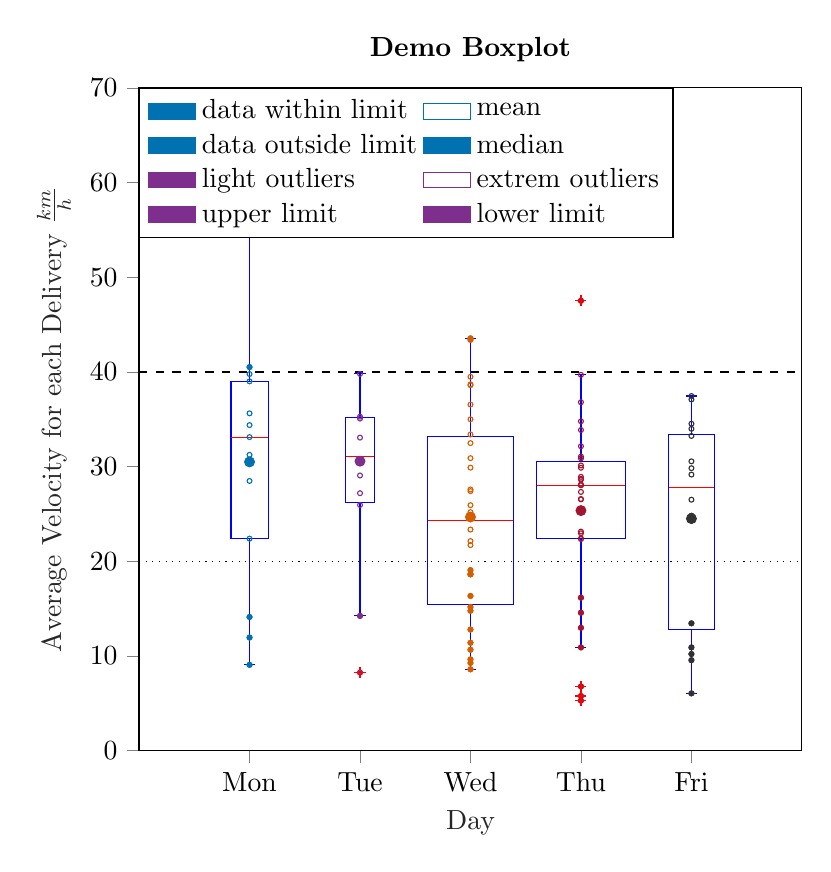
\begin{tikzpicture}

\begin{axis}[%
xmin=0,
xmax=6,
xtick={1,2,3,4,5},
xticklabels={{Mon},{Tue},{Wed},{Thu},{Fri}},
tick align=outside,
xlabel style={font=\color{white!15!black}},
xlabel={Day},
ymin=0,
ymax=70,
ylabel style={font=\color{white!15!black}},
ylabel={Average Velocity for each Delivery $\frac{km}{h}$},
axis background/.style={fill=white},
title style={font=\bfseries},
title={Demo Boxplot},
x tick label style={/pgf/number format/.cd, fixed, fixed zerofill, precision=0, /tikz/.cd},
y tick label style={/pgf/number format/.cd, fixed, fixed zerofill, precision=0, /tikz/.cd},
xtick={1,2,3,4,5},
ytick={0,10,20,30,40,50,60,70},
ytick pos=left,
xtick pos=bottom,
/pgf/number format/.cd, set decimal separator={.},
/pgf/number format/.cd, 1000 sep={},
legend style={at={(0,1)}, anchor=north west},
legend cell align={left},
at={(0cm,0cm)},
height=10cm,
width=10cm,
legend columns=2,
]
\addplot[only marks, mark=*, mark options={}, mark size=1.7678pt, color=mycolor1, fill=mycolor1] table[row sep=crcr]{%
x	y\\
1	30.5024557265965\\
};
\addplot[only marks, mark=o, mark options={}, mark size=0.8839pt, draw=mycolor1] table[row sep=crcr]{%
x	y\\
1	39.0084815114874\\
1	34.3890288272367\\
1	22.3970658616155\\
1	31.2480140486477\\
1	14.1238708482975\\
1	28.4907614227917\\
1	11.9581891623483\\
1	40.5165266583494\\
1	56.7943432997721\\
1	35.6316606505577\\
1	39.7812570008893\\
1	9.07203572475352\\
1	33.1206894290073\\
};
\addplot[only marks, mark=*, mark options={}, mark size=0.8839pt, color=mycolor1, fill=mycolor1] table[row sep=crcr]{%
x	y\\
1	14.1238708482975\\
1	11.9581891623483\\
1	9.07203572475352\\
};
\addplot[only marks, mark=*, mark options={}, mark size=0.8839pt, color=mycolor1, fill=mycolor1] table[row sep=crcr]{%
x	y\\
1	40.5165266583494\\
1	56.7943432997721\\
};
\addplot[only marks, mark=*, mark options={}, mark size=1.7678pt, color=mycolor6, fill=mycolor6] table[row sep=crcr]{%
x	y\\
2	30.5725475823818\\
};
\addplot[only marks, mark=o, mark options={}, mark size=0.8839pt, draw=mycolor6] table[row sep=crcr]{%
x	y\\
2	33.0622836365225\\
2	29.0699169678159\\
2	25.9464313313546\\
2	8.25735220975745\\
2	35.0762959817225\\
2	27.1979058718029\\
2	14.2417000475158\\
2	57.800890604846\\
2	39.7937496612021\\
2	35.2789495112784\\
};
\addplot[only marks, mark=*, mark options={}, mark size=0.8839pt, color=mycolor6, fill=mycolor6] table[row sep=crcr]{%
x	y\\
2	8.25735220975745\\
2	14.2417000475158\\
};
\addplot[only marks, mark=*, mark options={}, mark size=0.8839pt, color=mycolor6, fill=mycolor6] table[row sep=crcr]{%
x	y\\
2	57.800890604846\\
};
\addplot[only marks, mark=*, mark options={}, mark size=1.7678pt, color=mycolor10, fill=mycolor10] table[row sep=crcr]{%
x	y\\
3	24.6787608381139\\
};
\addplot[only marks, mark=o, mark options={}, mark size=0.8839pt, draw=mycolor10] table[row sep=crcr]{%
x	y\\
3	15.1855374294428\\
3	34.9998372633058\\
3	22.1450415635892\\
3	11.4048206766703\\
3	25.1977119082488\\
3	27.5894483422346\\
3	38.6015447724876\\
3	9.27420901243929\\
3	25.9311081569927\\
3	32.4864710112777\\
3	43.551328311405\\
3	12.8010634605193\\
3	21.7133774784987\\
3	30.8986900700704\\
3	36.5577598264824\\
3	14.7813334048164\\
3	9.64786113824805\\
3	16.3455690720932\\
3	39.4903722996707\\
3	8.59851099626618\\
3	43.3934832820867\\
3	38.6938760474687\\
3	27.4146951086896\\
3	33.3932099040591\\
3	19.0778692098653\\
3	10.6649042008879\\
3	18.6311242408586\\
3	23.3589063556792\\
3	18.6383349948303\\
3	29.8948256042313\\
};
\addplot[only marks, mark=*, mark options={}, mark size=0.8839pt, color=mycolor10, fill=mycolor10] table[row sep=crcr]{%
x	y\\
3	15.1855374294428\\
3	11.4048206766703\\
3	9.27420901243929\\
3	12.8010634605193\\
3	14.7813334048164\\
3	9.64786113824805\\
3	16.3455690720932\\
3	8.59851099626618\\
3	19.0778692098653\\
3	10.6649042008879\\
3	18.6311242408586\\
3	18.6383349948303\\
};
\addplot[only marks, mark=*, mark options={}, mark size=0.8839pt, color=mycolor10, fill=mycolor10] table[row sep=crcr]{%
x	y\\
3	43.551328311405\\
3	43.3934832820867\\
};
\addplot[only marks, mark=*, mark options={}, mark size=1.7678pt, color=mycolor11, fill=mycolor11] table[row sep=crcr]{%
x	y\\
4	25.3635030036125\\
};
\addplot[only marks, mark=o, mark options={}, mark size=0.8839pt, draw=mycolor11] table[row sep=crcr]{%
x	y\\
4	26.5457508183276\\
4	22.9620196946173\\
4	22.4170498183967\\
4	28.9220131320084\\
4	26.5819308087156\\
4	31.0682156567211\\
4	28.6266241616772\\
4	39.6951263505587\\
4	47.5206065568059\\
4	28.7179498049683\\
4	28.050434913074\\
4	30.8704896932798\\
4	5.2921221018118\\
4	22.3497076291235\\
4	34.7899749966156\\
4	12.9846556756357\\
4	36.7993109041144\\
4	33.87081654398\\
4	28.0434088645162\\
4	6.79060715167152\\
4	32.1537921241552\\
4	5.77629941370808\\
4	25.2115656068499\\
4	10.9095869303994\\
4	30.127692369124\\
4	27.3302805160142\\
4	28.0954444480632\\
4	16.1620595049288\\
4	23.145367939768\\
4	29.8825322238841\\
4	14.5751567584742\\
};
\addplot[only marks, mark=*, mark options={}, mark size=0.8839pt, color=mycolor11, fill=mycolor11] table[row sep=crcr]{%
x	y\\
4	5.2921221018118\\
4	12.9846556756357\\
4	6.79060715167152\\
4	5.77629941370808\\
4	10.9095869303994\\
4	16.1620595049288\\
4	14.5751567584742\\
};
\addplot[only marks, mark=*, mark options={}, mark size=0.8839pt, color=mycolor11, fill=mycolor11] table[row sep=crcr]{%
x	y\\
4	47.5206065568059\\
};
\addplot[only marks, mark=*, mark options={}, mark size=1.7678pt, color=mycolor12, fill=mycolor12] table[row sep=crcr]{%
x	y\\
5	24.5140405411153\\
};
\addplot[only marks, mark=o, mark options={}, mark size=0.8839pt, draw=mycolor12] table[row sep=crcr]{%
x	y\\
5	30.5639793754756\\
5	37.0954766098587\\
5	33.9940623901879\\
5	26.5104817331448\\
5	10.2154825905258\\
5	6.05574071842015\\
5	29.8399248058694\\
5	37.4557368539493\\
5	34.5330569785263\\
5	13.4568014655283\\
5	33.242341471018\\
5	24.8012242914818\\
5	24.8228470767842\\
5	10.9096701022062\\
5	29.1633726706225\\
5	9.56444952424545\\
};
\addplot[only marks, mark=*, mark options={}, mark size=0.8839pt, color=mycolor12, fill=mycolor12] table[row sep=crcr]{%
x	y\\
5	10.2154825905258\\
5	6.05574071842015\\
5	13.4568014655283\\
5	10.9096701022062\\
5	9.56444952424545\\
};
\addplot[only marks, mark=*, mark options={}, mark size=0.8839pt, color=mycolor12, fill=mycolor12] table[row sep=crcr]{%
x	y\\
};
\addplot [color=black, dashed]
  table[row sep=crcr]{%
0	40\\
6	40\\
};
\addplot [color=black, dotted]
  table[row sep=crcr]{%
0	20\\
6	20\\
};
\addplot [color=blue]
  table[row sep=crcr]{%
0.832258064516129	33.1206894290073\\
0.832258064516129	39.0084815114874\\
0.832258064516129	39.0084815114874\\
1.16774193548387	39.0084815114874\\
1.16774193548387	39.0084815114874\\
1.16774193548387	33.1206894290073\\
1.16774193548387	25.8874203453655\\
1.16774193548387	22.3970658616155\\
0.832258064516129	22.3970658616155\\
0.832258064516129	25.8874203453655\\
0.832258064516129	33.1206894290073\\
};
\addplot [color=blue]
  table[row sep=crcr]{%
1.87096774193548	31.0661003021692\\
1.87096774193548	35.2282861288894\\
1.87096774193548	35.2282861288894\\
2.12903225806452	35.2282861288894\\
2.12903225806452	35.2282861288894\\
2.12903225806452	31.0661003021692\\
2.12903225806452	26.6131996437704\\
2.12903225806452	26.2592999664667\\
1.87096774193548	26.2592999664667\\
1.87096774193548	26.6131996437704\\
1.87096774193548	31.0661003021692\\
};
\addplot [color=blue]
  table[row sep=crcr]{%
2.61290322580645	24.278309131964\\
2.61290322580645	29.3492776304138\\
2.61290322580645	33.1665251808637\\
3.38709677419355	33.1665251808637\\
3.38709677419355	29.3492776304138\\
3.38709677419355	24.278309131964\\
3.38709677419355	19.2073406335142\\
3.38709677419355	15.4755453401054\\
2.61290322580645	15.4755453401054\\
2.61290322580645	19.2073406335142\\
2.61290322580645	24.278309131964\\
};
\addplot [color=blue]
  table[row sep=crcr]{%
3.6	28.0434088645162\\
3.6	30.3318800519367\\
3.6	30.4990910312019\\
4.4	30.4990910312019\\
4.4	30.3318800519367\\
4.4	28.0434088645162\\
4.4	25.7549376770956\\
4.4	22.3833787237601\\
3.6	22.3833787237601\\
3.6	25.7549376770956\\
3.6	28.0434088645162\\
};
\addplot [color=blue]
  table[row sep=crcr]{%
4.79354838709677	27.8369272018837\\
4.79354838709677	33.4302717008104\\
4.79354838709677	33.4302717008104\\
5.20645161290323	33.4302717008104\\
5.20645161290323	33.4302717008104\\
5.20645161290323	27.8369272018837\\
5.20645161290323	19.7474028695095\\
5.20645161290323	12.8200186246978\\
4.79354838709677	12.8200186246978\\
4.79354838709677	19.7474028695095\\
4.79354838709677	27.8369272018837\\
};
\addplot [color=blue]
  table[row sep=crcr]{%
1	9.07203572475352\\
1	22.3970658616155\\
};
\addplot [color=blue]
  table[row sep=crcr]{%
2	14.2417000475158\\
2	26.2592999664667\\
};
\addplot [color=blue]
  table[row sep=crcr]{%
3	8.59851099626618\\
3	15.4755453401054\\
};
\addplot [color=blue]
  table[row sep=crcr]{%
4	10.9095869303994\\
4	22.3833787237601\\
};
\addplot [color=blue]
  table[row sep=crcr]{%
5	6.05574071842015\\
5	12.8200186246978\\
};
\addplot [color=blue]
  table[row sep=crcr]{%
1	56.7943432997721\\
1	39.0084815114874\\
};
\addplot [color=blue]
  table[row sep=crcr]{%
2	39.7937496612021\\
2	35.2282861288894\\
};
\addplot [color=blue]
  table[row sep=crcr]{%
3	43.551328311405\\
3	33.1665251808637\\
};
\addplot [color=blue]
  table[row sep=crcr]{%
4	39.6951263505587\\
4	30.4990910312019\\
};
\addplot [color=blue]
  table[row sep=crcr]{%
5	37.4557368539493\\
5	33.4302717008104\\
};
\addplot [color=blue]
  table[row sep=crcr]{%
0.95	9.07203572475352\\
1.05	9.07203572475352\\
};
\addplot [color=blue]
  table[row sep=crcr]{%
1.95	14.2417000475158\\
2.05	14.2417000475158\\
};
\addplot [color=blue]
  table[row sep=crcr]{%
2.95	8.59851099626618\\
3.05	8.59851099626618\\
};
\addplot [color=blue]
  table[row sep=crcr]{%
3.95	10.9095869303994\\
4.05	10.9095869303994\\
};
\addplot [color=blue]
  table[row sep=crcr]{%
4.95	6.05574071842015\\
5.05	6.05574071842015\\
};
\addplot [color=blue]
  table[row sep=crcr]{%
0.95	56.7943432997721\\
1.05	56.7943432997721\\
};
\addplot [color=blue]
  table[row sep=crcr]{%
1.95	39.7937496612021\\
2.05	39.7937496612021\\
};
\addplot [color=blue]
  table[row sep=crcr]{%
2.95	43.551328311405\\
3.05	43.551328311405\\
};
\addplot [color=blue]
  table[row sep=crcr]{%
3.95	39.6951263505587\\
4.05	39.6951263505587\\
};
\addplot [color=blue]
  table[row sep=crcr]{%
4.95	37.4557368539493\\
5.05	37.4557368539493\\
};
\addplot [color=red]
  table[row sep=crcr]{%
0.832258064516129	33.1206894290073\\
1.16774193548387	33.1206894290073\\
};
\addplot [color=red]
  table[row sep=crcr]{%
1.87096774193548	31.0661003021692\\
2.12903225806452	31.0661003021692\\
};
\addplot [color=red]
  table[row sep=crcr]{%
2.61290322580645	24.278309131964\\
3.38709677419355	24.278309131964\\
};
\addplot [color=red]
  table[row sep=crcr]{%
3.6	28.0434088645162\\
4.4	28.0434088645162\\
};
\addplot [color=red]
  table[row sep=crcr]{%
4.79354838709677	27.8369272018837\\
5.20645161290323	27.8369272018837\\
};
\addplot [color=red, draw=none, mark=+, mark options={solid, red}]
  table[row sep=crcr]{%
2	8.25735220975745\\
2	57.800890604846\\
4	47.5206065568059\\
4	5.2921221018118\\
4	6.79060715167152\\
4	5.77629941370808\\
};
\addlegendimage{only marks, black, mark=o, mark size=0.88388pt}
\addlegendentry{data within limit}
\addlegendimage{only marks, black, mark=*, mark size=1.7678}
\addlegendentry{mean}
\addlegendimage{only marks, black, mark=*, mark size=0.88388pt}
\addlegendentry{data outside limit}
\addlegendimage{line legend, red}
\addlegendentry{median}
\addlegendimage{only marks, red,mark=+, mark size=2pt}
\addlegendentry{light outliers}
\addlegendimage{only marks, red, mark=o, mark size=2pt}
\addlegendentry{extrem outliers}
\addlegendimage{line legend, black, dashed}
\addlegendentry{upper limit}
\addlegendimage{line legend, black, dotted}
\addlegendentry{lower limit}
\end{axis}
\end{tikzpicture}%
	\caption[Example 4: Boxplot]
	{
		A boxplot with grouping and data highlighting.
	}
\end{figure}

\lipsum[1-2]
\pagebreak
\lstinputlisting[caption={eeeee}, label=Beispiel5]{Beispiel5.m}

\begin{figure}[H]
	\centering
	% This file was created by matlab2tikz.%
%
\definecolor{mycolor1}{rgb}{0.00000,0.44706,0.69804}%
\definecolor{mycolor2}{rgb}{0.00000,0.44700,0.74100}%
\definecolor{mycolor3}{rgb}{0.85000,0.32500,0.09800}%
\definecolor{mycolor4}{rgb}{0.90196,0.62353,0.00000}%
\definecolor{mycolor5}{rgb}{0.92900,0.69400,0.12500}%
\definecolor{mycolor6}{rgb}{0.49400,0.18400,0.55600}%
\definecolor{mycolor7}{rgb}{0.00000,0.61961,0.45098}%
\definecolor{mycolor8}{rgb}{0.46600,0.67400,0.18800}%
\definecolor{mycolor9}{rgb}{0.30100,0.74500,0.93300}%
\definecolor{mycolor10}{rgb}{0.83529,0.36863,0.00000}%
\definecolor{mycolor11}{rgb}{0.63500,0.07800,0.18400}%
\definecolor{mycolor12}{rgb}{0.19608,0.19608,0.19608}%
%
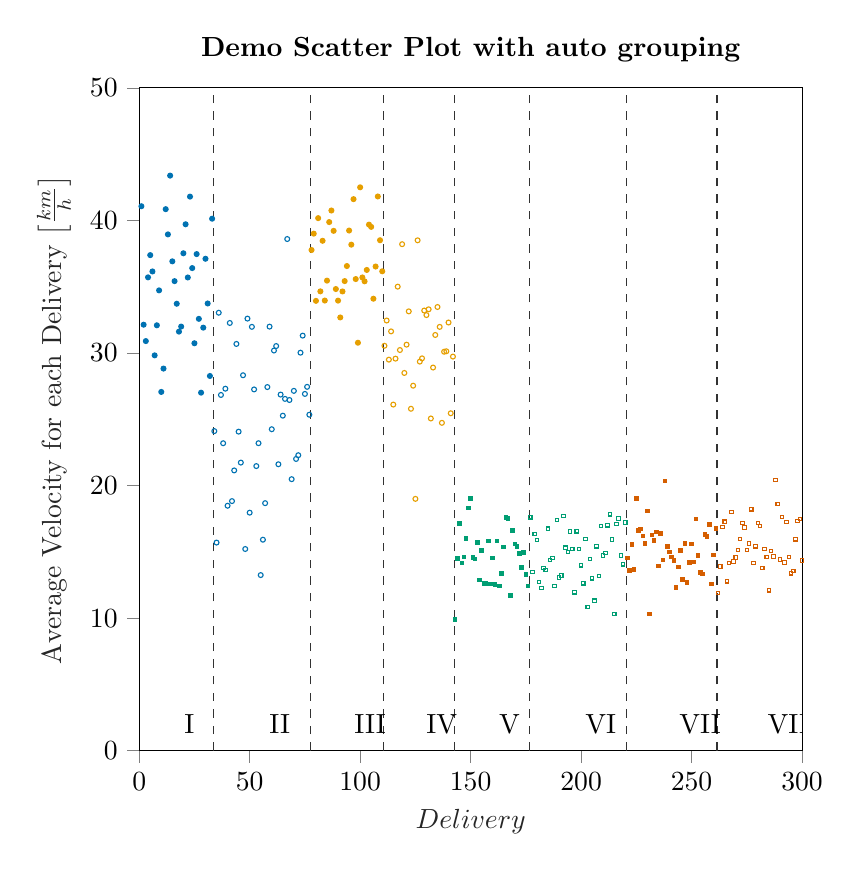
\begin{tikzpicture}

\begin{axis}[%
xmin=0,
xmax=300,
tick align=outside,
xlabel style={font=\color{white!15!black}},
xlabel={$Delivery$},
ymin=0,
ymax=50,
ylabel style={font=\color{white!15!black}},
ylabel={Average Velocity for each Delivery $\left[\frac{km}{h}\right]$},
axis background/.style={fill=white},
title style={font=\bfseries},
title={Demo Scatter Plot with auto grouping},
x tick label style={/pgf/number format/.cd, fixed, fixed zerofill, precision=0, /tikz/.cd},
y tick label style={/pgf/number format/.cd, fixed, fixed zerofill, precision=0, /tikz/.cd},
xtick={0,50,100,150,200,250,300},
ytick={0,10,20,30,40,50},
ytick pos=left,
xtick pos=bottom,
/pgf/number format/.cd, set decimal separator={.},
/pgf/number format/.cd, 1000 sep={},
legend style={at={(0,1)}, anchor=north west},
legend cell align={left},
at={(0cm,0cm)},
height=10cm,
width=10cm
]
\addplot[only marks, mark=*, mark options={}, mark size=0.8839pt, color=mycolor1, fill=mycolor1] table[row sep=crcr]{%
x	y\\
1	41.0715412018992\\
2	32.1354484355608\\
3	30.8998795488627\\
4	35.7084496512089\\
5	37.3840338508915\\
6	36.1519096933132\\
7	29.823363771372\\
8	32.0917024857327\\
9	34.7249668602181\\
10	27.064739545416\\
11	28.827007513992\\
12	40.8506508096863\\
13	38.948051031077\\
14	43.3815116880465\\
15	36.9149273831376\\
16	35.4229493693753\\
17	33.7172831243359\\
18	31.6136224400641\\
19	31.993987704071\\
20	37.5241039892991\\
21	39.7111097894575\\
22	35.6979854014755\\
23	41.7969337925032\\
24	36.406514358049\\
25	30.7365528205198\\
26	37.4630569734503\\
27	32.5778128314509\\
28	27.0088089590363\\
29	31.9135072090831\\
30	37.1098413636742\\
31	33.7376268258828\\
32	28.2685685096855\\
33	40.1311147616901\\
};
\addplot[only marks, mark=o, mark options={}, mark size=0.8839pt, draw=mycolor1] table[row sep=crcr]{%
x	y\\
34	24.1097740589294\\
35	15.7018926097384\\
36	33.0391287872755\\
37	26.8365014083176\\
38	23.1946835167388\\
39	27.3080828901977\\
40	18.4801159213395\\
41	32.2658222148215\\
42	18.8307350954099\\
43	21.1444223651186\\
44	30.6848199903182\\
45	24.067956561805\\
46	21.7340011109064\\
47	28.3235335358626\\
48	15.2172313936224\\
49	32.5964114560848\\
50	17.9574043036894\\
51	31.9742025821054\\
52	27.2532374290022\\
53	21.4722787486503\\
54	23.1972395657912\\
55	13.2499913160925\\
56	15.9178163322404\\
57	18.6741502676917\\
58	27.431841570523\\
59	31.9905533337273\\
60	24.2515382113654\\
61	30.1883186130559\\
62	30.5260717077989\\
63	21.6090139319383\\
64	26.8649496366504\\
65	25.2735231650584\\
66	26.5402972264909\\
67	38.5980066899913\\
68	26.4562860050875\\
69	20.483977286247\\
70	27.1449661001459\\
71	22.0090925648951\\
72	22.2924961096509\\
73	30.0251376147094\\
74	31.311577091629\\
75	26.915803997355\\
76	27.4487653026776\\
77	25.3457311930215\\
};
\addplot[only marks, mark=*, mark options={}, mark size=0.8839pt, color=mycolor4, fill=mycolor4] table[row sep=crcr]{%
x	y\\
78	37.7698057079744\\
79	39.0048814666916\\
80	33.9359281177381\\
81	40.1742098993096\\
82	34.6507413350551\\
83	38.4658032300711\\
84	33.9582693377563\\
85	35.460460222375\\
86	39.8768024431226\\
87	40.7495620609831\\
88	39.2149412265345\\
89	34.8265001743974\\
90	33.9510012096901\\
91	32.6829705418013\\
92	34.6436691847557\\
93	35.4276076926954\\
94	36.5606970430796\\
95	39.2386665943589\\
96	38.1735796430374\\
97	41.607019505093\\
98	35.5796418779491\\
99	30.7765732002543\\
100	42.4992903709581\\
101	35.6990983088888\\
102	35.4097104948359\\
103	36.2651304863228\\
104	39.6856083383723\\
105	39.5150009555391\\
106	34.0961442434814\\
107	36.524628724445\\
108	41.807598310858\\
109	38.5078073168363\\
110	36.1635940871953\\
};
\addplot[only marks, mark=o, mark options={}, mark size=0.8839pt, draw=mycolor4] table[row sep=crcr]{%
x	y\\
111	30.5464418339888\\
112	32.4518252356102\\
113	29.4995318808552\\
114	31.6319494534137\\
115	26.1109389625856\\
116	29.5763286030897\\
117	35.0060400031908\\
118	30.2250208660826\\
119	38.2084409771819\\
120	28.4962058505408\\
121	30.6295035668897\\
122	33.1417138443841\\
123	25.7944591625082\\
124	27.5351709983262\\
125	18.9986725628675\\
126	38.5013183431529\\
127	29.3523007597412\\
128	29.5989306051145\\
129	33.2039819625091\\
130	32.8626920135185\\
131	33.2977619878003\\
132	25.0624855912505\\
133	28.9043620992219\\
134	31.3618412989036\\
135	33.4704511417714\\
136	31.9706675691597\\
137	24.7343833588576\\
138	30.0969000526069\\
139	30.1320874323086\\
140	32.3009911840212\\
141	25.4552781650928\\
142	29.7307933028643\\
};
\addplot[only marks, mark=square*, mark options={}, mark size=0.6250pt, color=mycolor7, fill=mycolor7] table[row sep=crcr]{%
x	y\\
143	9.90281248272419\\
144	14.5044796460759\\
145	17.1347247869069\\
146	14.1651623280268\\
147	14.6069687393957\\
148	16.017984811054\\
149	18.3218082405726\\
150	19.0271904138155\\
151	14.5741116137586\\
152	14.4790425993493\\
153	15.6985981738054\\
154	12.869146082907\\
155	15.109632947651\\
156	12.613058940901\\
157	12.6006872417458\\
158	15.8342358230293\\
159	12.5770791563507\\
160	14.5451962834924\\
161	12.5399570039255\\
162	15.8275337442787\\
163	12.429156433922\\
164	13.3503629746016\\
165	15.3795626333762\\
166	17.5999038249665\\
167	17.5381176988081\\
168	11.7251988623569\\
169	16.6049215925074\\
170	15.6062252920075\\
171	15.4196825602957\\
172	14.897209482416\\
173	13.8100405892121\\
174	14.9625538762796\\
175	13.3006855780162\\
176	12.4406611011627\\
};
\addplot[only marks, mark=square, mark options={}, mark size=0.6250pt, draw=mycolor7] table[row sep=crcr]{%
x	y\\
177	17.6093015558749\\
178	13.4891455635951\\
179	16.3418099421068\\
180	15.9000766442167\\
181	12.7396447157021\\
182	12.2785530450832\\
183	13.7851627595725\\
184	13.6222749832595\\
185	16.7498842962424\\
186	14.3907779975709\\
187	14.5248809157676\\
188	12.4328527445116\\
189	17.4064904126351\\
190	13.057256596948\\
191	13.224471821177\\
192	17.7112295193351\\
193	15.3164653022037\\
194	15.0050164595186\\
195	16.5356805001386\\
196	15.2027773114287\\
197	11.9508324437773\\
198	16.5550211076371\\
199	15.2221964090874\\
200	13.9875017829299\\
201	12.6358214571321\\
202	15.9677902406051\\
203	10.8433879563136\\
204	14.4509148106817\\
205	13.0083958282834\\
206	11.3162134670654\\
207	15.4262267515209\\
208	13.190374766673\\
209	16.9476615503682\\
210	14.7353673549844\\
211	14.9223253572628\\
212	17.0049757596276\\
213	17.8340090984653\\
214	15.9434420125002\\
215	10.3140517248115\\
216	17.1057087248657\\
217	17.5077994955526\\
218	14.7375912673249\\
219	14.0664517554208\\
220	17.2274349345557\\
};
\addplot[only marks, mark=square*, mark options={}, mark size=0.6250pt, color=mycolor10, fill=mycolor10] table[row sep=crcr]{%
x	y\\
221	14.5353160322745\\
222	13.6051406883932\\
223	15.5527138815372\\
224	13.6873800052146\\
225	19.0064414734292\\
226	16.604767883189\\
227	16.726388048541\\
228	16.2072968591893\\
229	15.6242247140068\\
230	18.0887235830685\\
231	10.3057782695203\\
232	16.2695625932249\\
233	15.8659614729793\\
234	16.4866498111095\\
235	13.9208646845208\\
236	16.3920666405182\\
237	14.3748903790268\\
238	20.3610120548695\\
239	15.4224471909674\\
240	15.00059506081\\
241	14.6052199476063\\
242	14.3464073401143\\
243	12.3143214056492\\
244	13.8605623015822\\
245	15.0848091202436\\
246	12.9024438528668\\
247	15.6386861208023\\
248	12.6801929295661\\
249	14.2085810494061\\
250	15.5948914152927\\
251	14.2500311374446\\
252	17.4741956310901\\
253	14.7143550682599\\
254	13.4633276394117\\
255	13.347174567719\\
256	16.3162458293507\\
257	16.1408268245409\\
258	17.0752448260407\\
259	12.592533630509\\
260	14.7597681769944\\
261	16.7464694871346\\
};
\addplot[only marks, mark=square, mark options={}, mark size=0.6250pt, draw=mycolor10] table[row sep=crcr]{%
x	y\\
262	11.8876124676239\\
263	13.9054254062569\\
264	16.8791128595339\\
265	17.2702719600854\\
266	12.7801039315652\\
267	14.1487629534708\\
268	18.0082370415004\\
269	14.2722221546478\\
270	14.5786402244664\\
271	15.1565160508687\\
272	15.9562546464443\\
273	17.1765418852997\\
274	16.847870925081\\
275	15.1442132117937\\
276	15.6189084652375\\
277	18.2113598424361\\
278	14.1556347281695\\
279	15.4262953562222\\
280	17.1875709946975\\
281	16.9677203096475\\
282	13.7883750819429\\
283	15.2226855224725\\
284	14.6244025979839\\
285	12.1012065910751\\
286	15.0510408675435\\
287	14.6605727934013\\
288	20.4087025002205\\
289	18.6049935157645\\
290	14.4243307963828\\
291	17.6450474178942\\
292	14.206924049933\\
293	17.2602602347549\\
294	14.6083486459811\\
295	13.3832626690275\\
296	13.562883178932\\
297	15.9470696446838\\
298	17.3252099137172\\
299	17.484390142621\\
300	14.3436946520175\\
};
\addplot [color=mycolor12, dashed, forget plot]
  table[row sep=crcr]{%
33.5	0\\
33.5	50\\
};
\addplot [color=mycolor12, dashed, forget plot]
  table[row sep=crcr]{%
77.5	0\\
77.5	50\\
};
\addplot [color=mycolor12, dashed, forget plot]
  table[row sep=crcr]{%
110.5	0\\
110.5	50\\
};
\addplot [color=mycolor12, dashed, forget plot]
  table[row sep=crcr]{%
142.5	0\\
142.5	50\\
};
\addplot [color=mycolor12, dashed, forget plot]
  table[row sep=crcr]{%
176.5	0\\
176.5	50\\
};
\addplot [color=mycolor12, dashed, forget plot]
  table[row sep=crcr]{%
220.5	0\\
220.5	50\\
};
\addplot [color=mycolor12, dashed, forget plot]
  table[row sep=crcr]{%
261.5	0\\
261.5	50\\
};
\node[right, align=left]
at (axis cs:16,2) {I};
\node[right, align=left]
at (axis cs:54.5,2) {II};
\node[right, align=left]
at (axis cs:93,2) {III};
\node[right, align=left]
at (axis cs:125.5,2) {IV};
\node[right, align=left]
at (axis cs:158.5,2) {V};
\node[right, align=left]
at (axis cs:197.5,2) {VI};
\node[right, align=left]
at (axis cs:240,2) {VII};
\node[right, align=left]
at (axis cs:280,2) {VIII};
\end{axis}
\end{tikzpicture}%
	\caption[Example 5: Scatter]
	{
		A scatter plot with auto grouping
	}
\end{figure}
